\documentclass{article}
\usepackage{geometry}
\usepackage[utf8]{inputenc}
\usepackage{graphicx}
\graphicspath{ {images/} }
\geometry{a4paper, left=25mm, right=25mm, top=25mm, bottom=25mm}
\setlength{\parindent}{2em}
\setlength{\parskip}{1em}
\renewcommand{\baselinestretch}{1.3}
\usepackage{fancyhdr}
\pagestyle{fancy}
\fancyhf{}
\rhead{S.Goldie - 42611814}
\lhead{FOAR705 - Learning Journal}
\lfoot{Session 2, 2019 - Macquarie University}
\rfoot{Page \thepage}


% To hyperlink references in contents and other lists
\usepackage[colorlinks=true,linkcolor=blue]{hyperref}
\usepackage{hyperref}
% To create a list of labels
% https://tex.stackexchange.com/a/418302/5482
\usepackage{crossreftools}
% Apply filter to list of labels - so that labels from figures are not affected
\newcommand{\includelabelintoc}{Error:}


\title{FOAR705 - Digital Fundamentals}
\author{Sheriden Goldie}
\date{Session 2, Macquarie University}

\begin{document}

\maketitle

\section*{Data Carpentry Exercises}

% create table of contents based on sections/subsections
\tableofcontents

% Create and index of errors
% so the list has a pretty name
\renewcommand
\listoflabelsname{List of Errors}

\crtlistoflabels
\pagebreak

\section{Spreadsheets for Social Sciences}

It is important for researchers to observe good data practices when working with data to ensure that errors, corruption, and misrepresentation are kept to a minimum. 
Good data practices mean that if mistakes are made - they can be found, noticed, and rectified before any analysis is done. This saves time and frustration from the researchers, and those that hope to use their method or findings. 

\textbf{Initial Questions}
\begin{itemize}
    \item How many people have used spreadsheets in their research?
\end{itemize}

I haven't used spreadsheets for my research - but in my previous 'life' i worked in inventory planning and operations. This lead me to using spreadsheets everyday.

\begin{itemize}
    \item How many people have accidentally done something that made them frustrated or sad?
\end{itemize}

I have had the experience of someone messing up my model data for inventory sheets, that was an time-sink to find the issues and to fix. I have also accidentally applied formulas to the wrong cells, which gave me really weird results. 

\subsection{Formatting data tables in Spreadsheets}

\textbf{Responses to Questions}

\begin{enumerate}
    \item With the person next to you, identify what is wrong with this spreadsheet. Discuss the steps you would need to take to clean up the two tabs, and to put them all together in one spreadsheet.
\end{enumerate} 

There are many things wrong with this spreadsheet:
\begin{itemize}
    \item It is difficult that all the data is split across different tables in each tab - it is hard to tell if the studied locations overlap or not. 
    \item Terms in columns vary - eg. \begin{verbatim} mabati_sloping vs. mabatisloping
    \end{verbatim}
    \item Some data doesn't make sense - eg. -99 in the rooms column - this is not a full integer and is not a valid data point. 
    item\ Data tables are not the same in both tabs. There is a 'Plots' table in Mozambique tab, but not in the Tanzania tab.
    \item the highlighted cell is unclear as to the relevance of the additional barn
    \item the asterisk marked data to include a cowshed is unclear
    \item the asterisked data on cows is misleading as it adds the now dead cow to the count that should just be looking at the collected temporally fixed data
    \item the livestock table in the Mozambique tab is VERY problematic. It combines all data in one cell without defining the individual animal counts
    \item the Mozambique livestock table also includes the 'Look after Cows' column which is not consistent/relevant
    \item the livestock table in the Tanzania tab contains empty fields - is this a zero count, or a missing count?
    \item In the Tanzania tab there seems to be an inconsistency with the 'sunbricks' entry - is this different to burntbricks? - how are these forms being classified and named for the purpose of the study?
    \end{itemize}

\subsubsection{Metadata}
\textbf{A Note on Metadata}

Metadata is data about your data. This is the information that is going to tell you what the answer to a query that is in a column is in reply to. This is imperative as human memory is fallible, and you are likely to forget your intentions unless they are noted and recorded explicitly. 

Digital data is designed to be read by machines, but understanding the meaning of the data can only be done by humans, and this is the valuable part of the process. However your data should be understandable to other humans - for the reasons that they might need to try and replicate your results, or they may wish to replicate the model of your study, or even for their own project starting point - being able to understand the data is made more efficient with metadata. 

Considering metadata during both the collection and analysis phases of research is important, especially if your research is to become part of the scholarly record. 

\noindent \textbf{Questions}
\begin{itemize}
    \item Discuss this data with a partner and make a list of some of the types of metadata that should be recorded about this data set. It may be helpful to start by asking yourself, ``What is not immediately obvious to me about this data? What questions would I need to know the answers to in order to analyze and interpret this data?''
\end{itemize}

Types of metadata that should be recorded
\begin{itemize}
    \item The question or prompt that generated each type of response - eg: for no. of members - the question might be: How many people live in this household? or it might be how many people are in your family? these are distinctly different questions
    \item what the expected range or allowable response is - eg: numerical only, between 1-30, yes/no response only
    \item what the terms used in the data mean - eg: muddaub - means the walls are structured using mud daubed over straw. Or definitions like what a 'plot' or 'room' is being defined as. 
\end{itemize}

\subsection{Formatting Problems}

Other problems to consider is the formatting - using the ``mergecell'' function to make the data look ``pretty''.
As this is ``raw data'' its purpose is to organise the data in a way that is effective and able to be manipulated by the program to create relevant, interpret able outputs. 

\subsection{Dates as Data}
\textbf{Separating dates into components}
to do the exercise these are the processes/actions I took:
\begin{enumerate}
    \item Download file
    \item Open file using Microsoft Excel
    \item Identified table to manipulate
    \item Copied table to new sheet - labelled this sheet 'working tab'
    \item Added three columns between columns A and B using insert columns function. These are labelled 'Day', 'Month', and 'Year' respectively.
    \item Entered the following codes into cells b2: =DAY(A2) c2: =MONTH(A2) d2: =YEAR(A2)
    \item I formatted columns B, C, and D, to a number format without decimal places. 
    \item Adding a new line of data just with the 17/11 information meant the data in the year column automatically populated the current year - 2019. 
\end{enumerate}

\subsection{Quality Assurance}
The processes/actions I took:
\begin{enumerate}
    \item Download file
    \item Open file using Microsoft Excel
    \item Copied table to new sheet - labelled this sheet 'working tab'
    \item Select column D
    \item While column is highlighted go to File - Data - Data Tools - Data Validation
    \item In the section tab of the window use the drop-down menu under Allow to select 'Whole Number'.
    \item Under Data select 'between' and enter 1 as the minimum and 30 as the maximum. 
    \item To test this is working, I tried entering '31' in cell D133. I received an error message as expected. 
    \item Go back to the the Data Validation window. In the Input Error tab, I enter a custom input error name and description.
    \item Go back to the the Data Validation window. In the Error Alert tab select style: Warning and input a custom warning. Title: Invalid Entry. Error Message: Entry must be between 1 and 30.
    \item I created an additional rule set for column E. The age range was set as 0 - 120, it should be a whole number and the warning message was set as: Age should be in whole years and between 0 and 120.
    \item I applied an additional data validation to column F. This was to allow a selection from a list of accepted entries. 
    \item I went to the Data Validation Window while the column was selected. In the Setting's tab I selected the following: ``Allow'' was set to ``List''. with ``ignore blank'' and ``in cell dropdown'' checked. 
    \item Then in the ``Source'' field, I typed the entries, separated by a comma and a space. As so "grass, muddaub, burntbricks, sunbricks, cement"
    \item I entered the Input Error as, title: ``Entry must be as per List'', and Error message: ''The entry must be entered as per the following list: grass, muddaub, burntbricks, sunbricks, cement. Use the dropdown menu to select your entry''
    \item I also tried creating a table as the  ``Source'' data in an additional worksheet. This worked - however care must be taken as this would not be preserved if exporting the data to a .CSV file. 
\end{enumerate}

\subsection{Exporting Data}
Save a file in CSV format.
The steps/actions I took:
\begin{enumerate}
    \item Go to: File - Save As
    \item Select folder directory to save file to
    \item Name file and select .CSV as file format.
    \item Click save
    \item As I had created a new tab for my working data I was only able to save that tab as a CSV. This is good to know for purposes of separating raw data, working data, and for versioning and back up purposes as well. 
\end{enumerate}

\subsection{Reflections}
The Data Carpentry exercises were useful as they reminded me of the 'best practice' ways of dealing with data, and the ideals for how it should be recorded to maximise the potential output. 
In my previous  roles in Inventory Planning and Finance Administration, I have worked with data a lot in various settings and for various purposes - so the mechanics of this task was not new or difficult for me, and so I did not encounter any major issues. 
However the process of documenting my learning process concurrent with the activity of learning was new, and it was useful to think through each step of the process as a single function. 

\section{The Unix Shell}

The aim of this exercise is to gain familiarity with using a Unix Shell. 
I have heard of a Unix Shell before, and have seen one used to manage the data for a commission based sales system. However I have never used it, and am interested to see how it actually works. 

\subsection{Setup}
In the setup we download a zip file, and extract the files within it to the desktop. 
The next step is to open a 'terminal' and type a command. 

I am using windows and do not have a native terminal - so I need to download one. The lesson recommends Git for Windows. 

I go to the following website to download the software:
\begin{verbatim}
    https://gitforwindows.org/
\end{verbatim}

I am able to download, install, and open the software successfully. 

\subsection{Introducing the Shell}

We most commonly interact with computers through a \textbf{GUI}; a \textbf{G}raphic \textbf{U}ser \textbf{I}nterface. We can give instructions to a computer through a GUI by a few mouse clicks. While this model is quite intuitive and easy to learn (it has allowed us to become digitally immersed with little technical training), it doesn't scale well to large scale tasks.  

\textbf{The Shell} is a command line interface, (CLI). This is an interface that is based on "knowledge in the head", but is also able to complete repetitive tasks quickly and efficiently.

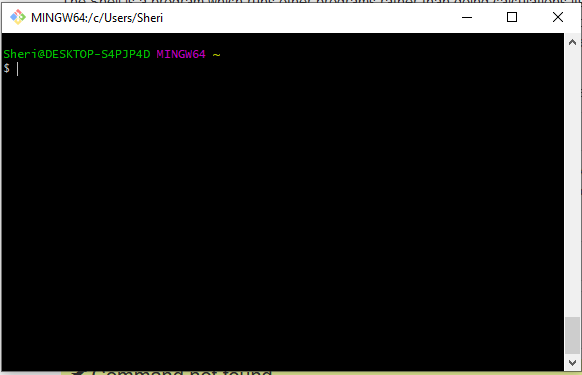
\includegraphics[width=10cm]{Images/GitBash_001.PNG}


The first symbol is \$ - this is a prompt, and means the shell is ready and waiting for you to type a command. 

The first command we try is: ls

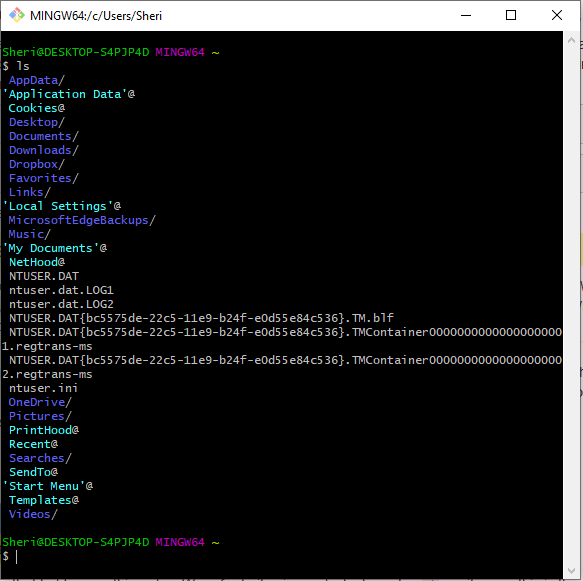
\includegraphics[width=10cm]{Images/GitBash_002.PNG}

This lists the contents of the \textbf{current} directory.
I am able to validate the list generated by the CLI by navigating to the folder using File Explorer in my GUI.
There are some things listed here in light blue that do not appear visibly in my GUI view of the same location.
Later notes indicate that an \@ means a link, an \* means an executable file, and a trailing / means that this is a directory.

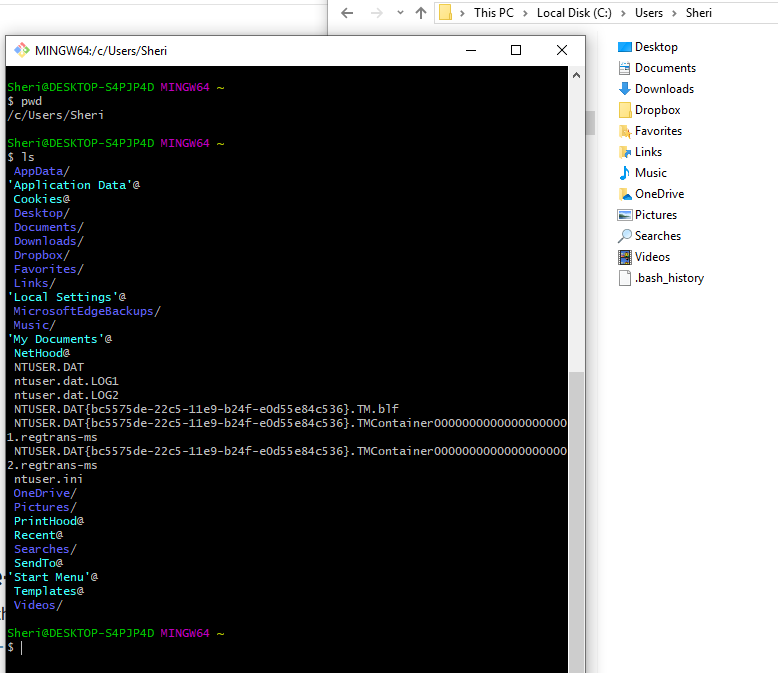
\includegraphics[width=10cm]{Images/GitBash_004.PNG}


\subsection{Navigating Files and Directories}

The first command I use is ``pwd''.
This tells us where we are currently "located in our system according to the CLI. This is important to know, so that we know what locations commands can and will be applied to.

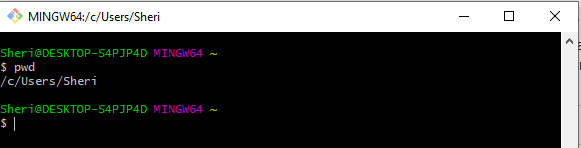
\includegraphics[width=10cm]{Images/GitBash_003.PNG}

\subsubsection{Syntax of a Command Line}
A command line is made up of component parts. For example the following command line: \$ ls -F /

\begin{itemize}
    \item \$ is the prompt beginning all lines in the CLI (At least within GitBash)
    \item ls is a LIST command, and tells the CLI to list everything in a directory
    \item -F is an option (also called a flag or switch) that changes what the command does - in this case it changes the format/colour output.
    \item / is an argument which is telling the command to look to the root directory (not the current directory) to create the list.
\end{itemize}

Options and arguments are also called parameters in some contexts.

Use command ls --help to bring up a list of options for the command. 

Trialling other options:
\begin{itemize}
    \item Command line: ls -l
    \item This creates the list using a ``long'' format. It includes other information about each file/folder.
\end{itemize}

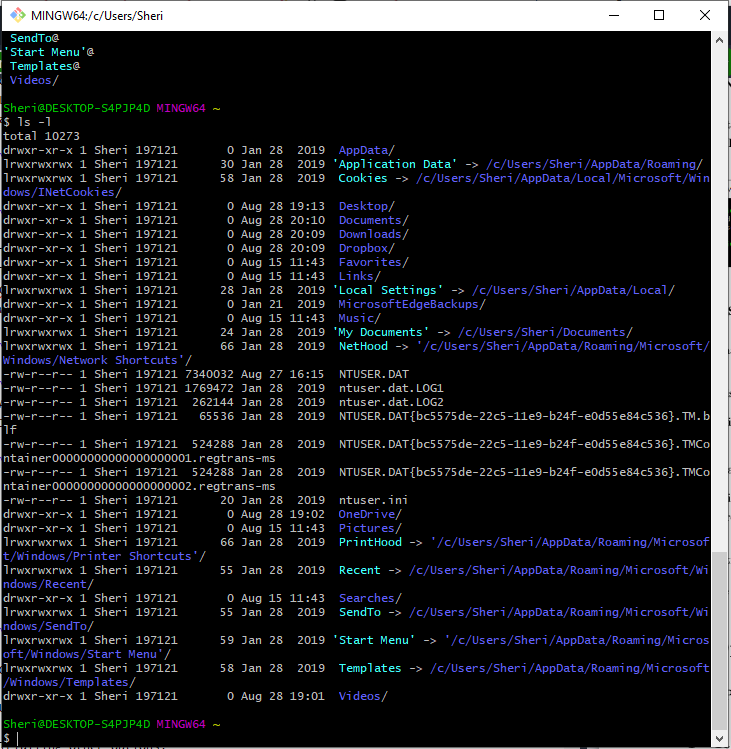
\includegraphics[width=10cm]{Images/GitBash_005.PNG}

\begin{itemize}
    \item Command line: ls -lh
    \item This uses the long list format but simplifies some data points to be more easily readable by a human. 
\end{itemize}

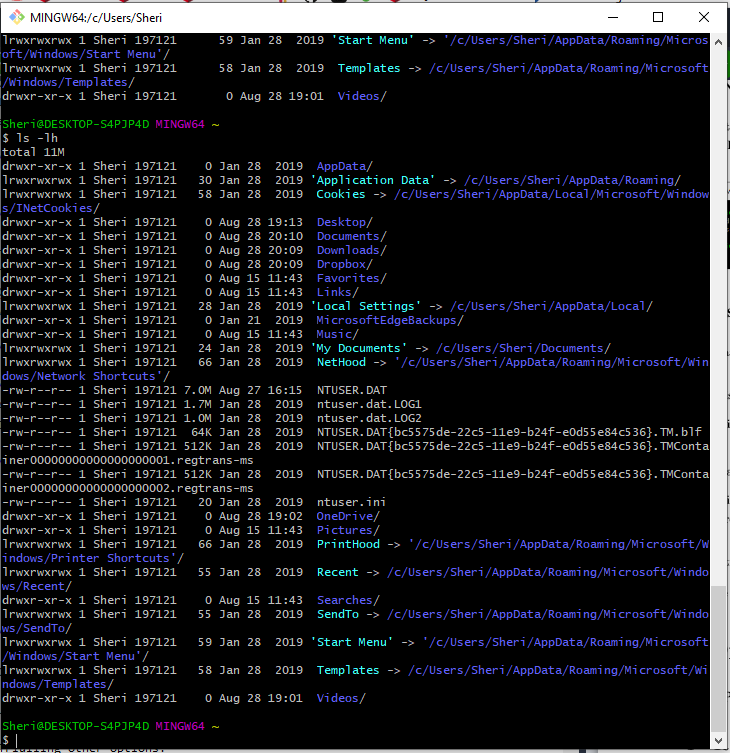
\includegraphics[width=10cm]{Images/GitBash_006.PNG}

The exercise also said to use command line: ls -R which will list the content of the directory recursively. 

When I ran this command - it took a long time to run, as it is listing every directory, and it sub directories and so on at each level. 

Using the option -t shows the list in a different order, based on the last modified folder. 

Next we try moving to different directories using command line: cd [folder location here].

Here cd means change directory - though it really means to change where the shell is considering the current directory to be.

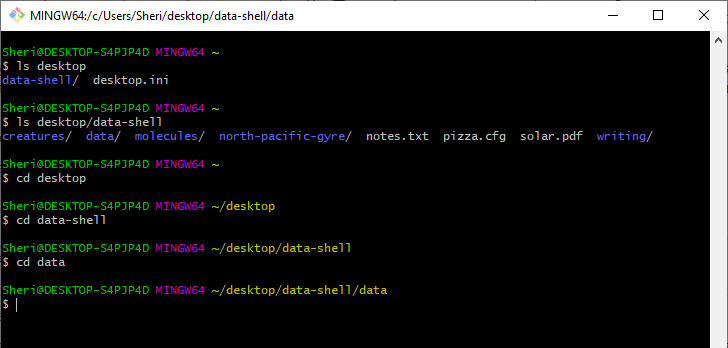
\includegraphics[width=10cm]{Images/GitBash_007.PNG}

Here we can use the pwd command to confirm where we are. Though in GitBash it shows an indication of this in the yellow text.

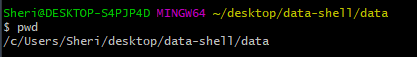
\includegraphics[width=10cm]{Images/GitBash_008.PNG}

If we want to move back through our directories - using cd as we have so far doesn't work, as without any other parameters it is only looking at sub-directories from its current position. 

To move back we use the command cd ..

Here the .. means "directory containing this one".

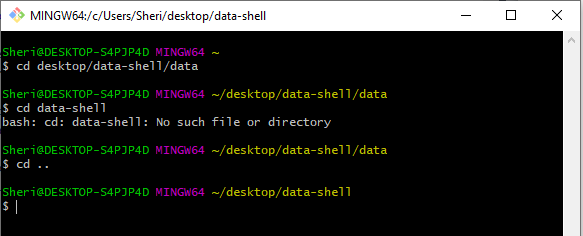
\includegraphics[width=10cm]{Images/GitBash_009.PNG}

We can also add the parameter -a to a ls command to show the indication of these parent directories.

We can also use command cd as a way to return to the root directory. This can then be confirmed by the pwd command.

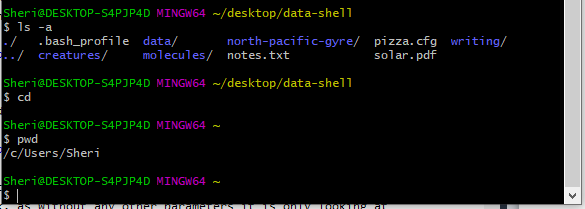
\includegraphics[width=10cm]{Images/GitBash_010.PNG}

Navigate back to the data directory, and validate that you are in the correct place:

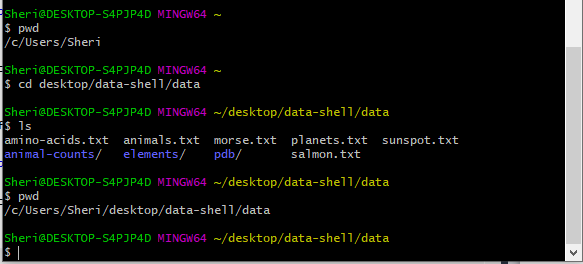
\includegraphics[width=10cm]{Images/GitBash_011.PNG}

\textbf{Other useful shortcuts}

The shell interprets the tilde character (\~{}) at the start of a path to mean ``the current user’s home directory''. For example, if Nelle’s home directory is /Users/nelle, then \~{}/data is equivalent to /Users/nelle/data. This only works if it is the first character in the path: here/there/~/elsewhere is not here/there/Users/nelle/elsewhere.

Another shortcut is the - (dash) character. cd will translate - into the previous directory I was in, which is faster than having to remember, then type, the full path. This is a very efficient way of moving back and forth between directories. The difference between cd .. and cd - is that the former brings you up, while the latter brings you back. You can think of it as the Last Channel button on a TV remote.

\subsubsection{Absolute vs Relative Paths}
So far, when specifying directory names, or even a directory path (as above), we have been using relative paths. When you use a relative path with a command like ls or cd, it tries to find that location from where we are, rather than from the root of the file system.

However, it is possible to specify the absolute path to a directory by including its entire path from the root directory, which is indicated by a leading slash. The leading / tells the computer to follow the path from the root of the file system, so it always refers to exactly one directory, no matter where we are when we run the command.

Source: http://swcarpentry.github.io/shell-novice/02-filedir/index.html

\subsection{Working With Files and Directories}

I first check I am still working in the data-shell directory

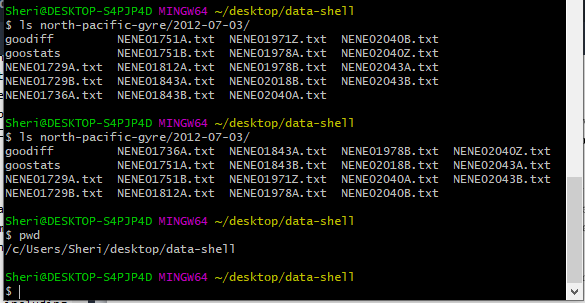
\includegraphics[width=10cm]{Images/GitBash_012.PNG}


\subsubsection{Creating Directories}

To create a new directory within the one we are in, we use the mkdir command:
Validate that the directory has been made using ls command.

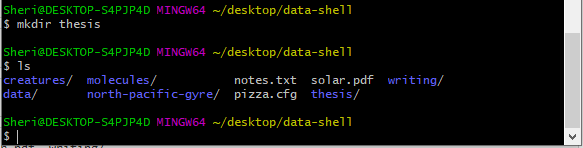
\includegraphics[width=10cm]{Images/GitBash_013.PNG}

\subsubsection{Good Naming Conventions}

For files that you will be using with the CLI - it is important to note that as a ``space'' is what separates commands and parameters, that having spaces in file and directory names is not ideal. Using hyphens, underscores, or using no spaces will make working with files in the CLI much easier.

\subsubsection{Creating a .txt File}

Change the working directory to the newly created ``Thesis'' folder. Create a text file using the command nano.

This will bring up a text editor. Enter some text and use ctrl+o to write the changes to the disc. Use ctrl+x to return to the command line.

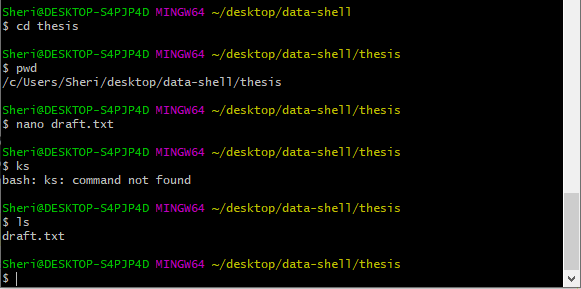
\includegraphics[width=10cm]{Images/GitBash_014.PNG}
\\*
\\*
\textbf{Creating a file a different way}

Try using the touch command to create a .txt file.

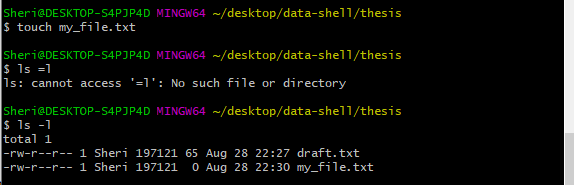
\includegraphics[width=10cm]{Images/GitBash_015.PNG}

This creates the file, but doesn't open the text editor. This creates an empty file. Which is useful for programs that might require a file to be created for it to input data into.

\subsection{Moving Files and Directories}
Return to the data-shell directory.

Change a the file called draft.txt using the mv command.
navigate to the thesis directory and validate that the file has changed names.

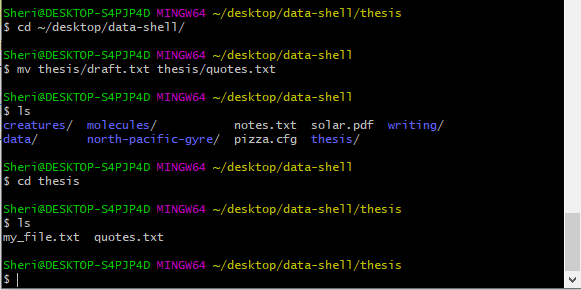
\includegraphics[width=10cm]{Images/GitBash_016.PNG}

Move the quotes.txt file to the current directory using the mv command.
NB: I had to move directories to do this step correctly.

\textbf{Using exact command in CLI error}
\label{ Error: Using exact commands in CLI}

Also including the period . was key for the command to work as this is a shorthand for the current directory.

One has to be careful when specifying the target file name, since mv will silently overwrite any existing file with the same name, which could lead to data loss. An additional option, mv -i (or mv --interactive), can be used to make mv ask you for confirmation before overwriting.

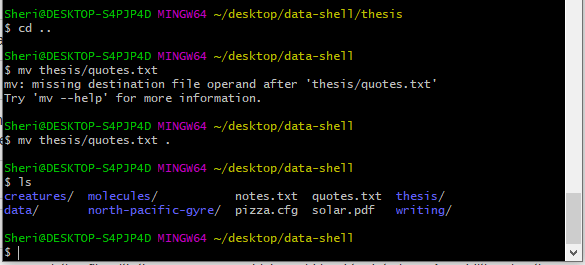
\includegraphics[width=10cm]{Images/GitBash_017.PNG}

\subsection{Copying Files}

Copy the quotes.txt file to the Thesis directory and rename it quotations.txt using the cp command.

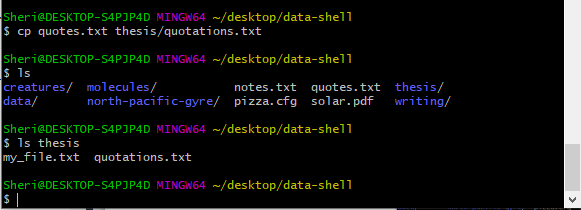
\includegraphics[width=10cm]{Images/GitBash_018.PNG}

You can use the same command on multiple locations in the shell:

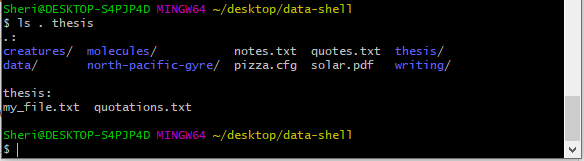
\includegraphics[width=10cm]{Images/GitBash_020.PNG}

Use a recursive option to copy a directory and all it's contents to a different directory.

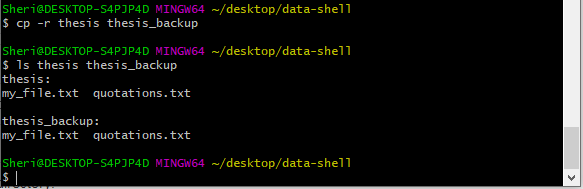
\includegraphics[width=10cm]{Images/GitBash_021.PNG}

\subsubsection{Removing Files and Directories}
Return to the data-shell directory and remove the quotes.txt file using the rm command.

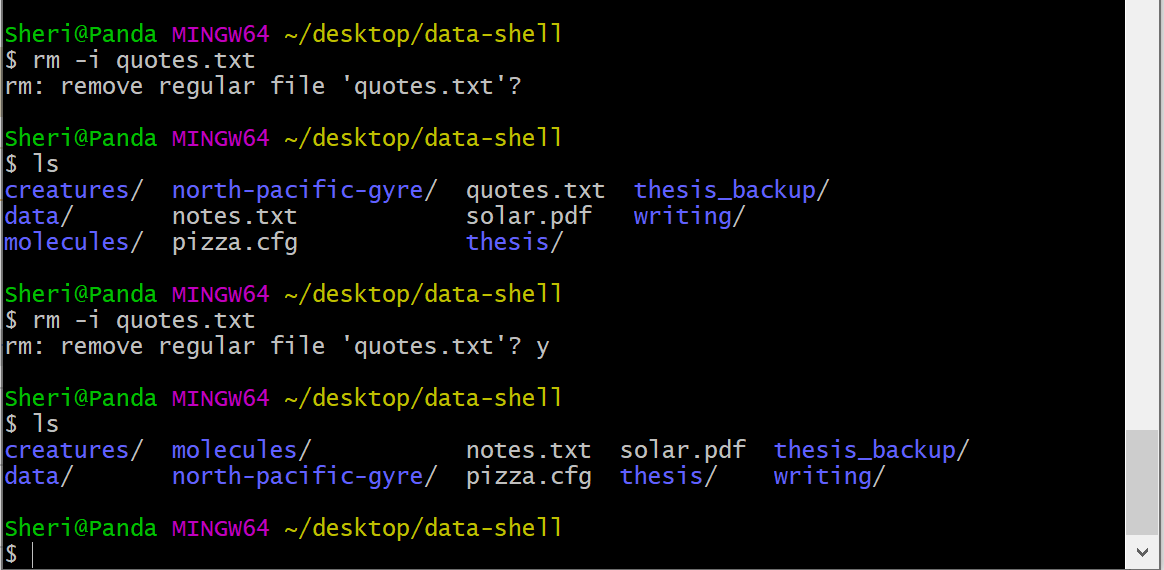
\includegraphics[width=10cm]{Images/GitBash_025.PNG}

\textbf{Shell Command rm -i Confirmation}
\label{ Error: Shell Command rm -i Confrimation}
When using the rm command with the -i parameter, it gives a second prompt to confirm if you want to complete the action. 

This requires a response - as just pressing enter negates the command. I responded by typing y, and this confirmed the command, and removed the file.

When trying to apply this same command to a directory we get an error message.
When using the command rm -ir we are asking to remove the files recursively. So the interface is able to interpret the intention to check/delete the files within the directory. Only when  the directory is empty can it be deleted.

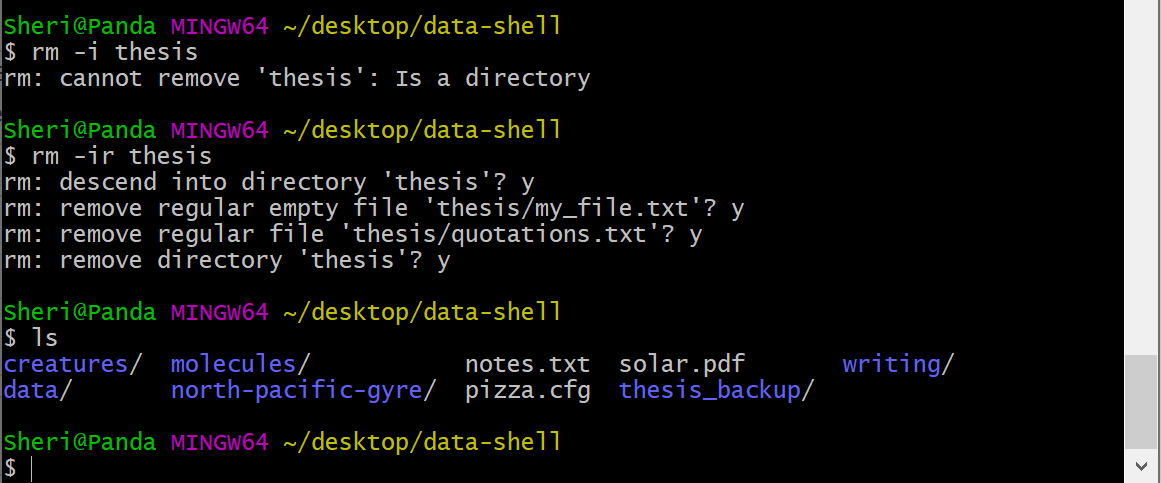
\includegraphics[width=10cm]{Images/GitBash_026.PNG}

\subsubsection{Wildcards}
* is a wildcard function that matches zero or more characters, while ? is a wildcard function that matches exactly one character.

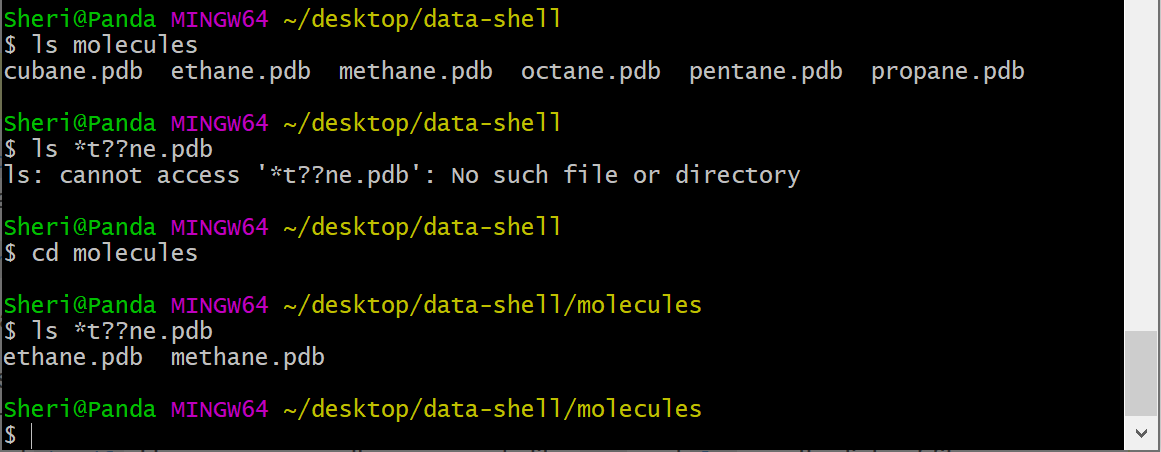
\includegraphics[width=10cm]{Images/GitBash_027.PNG}

\subsection{Pipes and Filters}
We discussed in class that GitBash, or similar Unix shells, are very good at doing individual tasks. The power of it becomes apparent when we are able to combine commands to create an output. This is like putting bits of pipe together, the output of one pipe, one command, can become the input for the next command. 

The first thing in this section is learning the wc command. This is for word count.

The first thing I do is navigate to the necessary location, and verify that I am in the correct place.

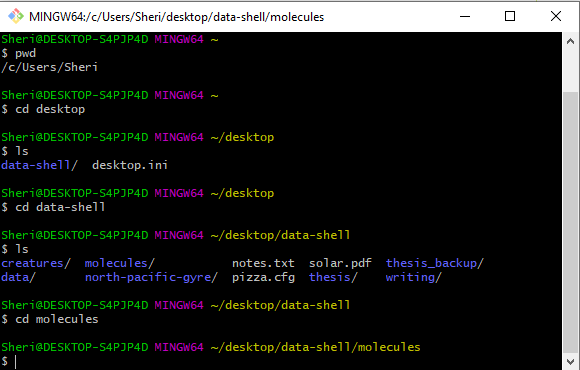
\includegraphics[width=10cm]{Images/GitBash_028.PNG}

The using the wc command, we are able to generate a list. The results from left to right read, line count, word count, character count, filename.

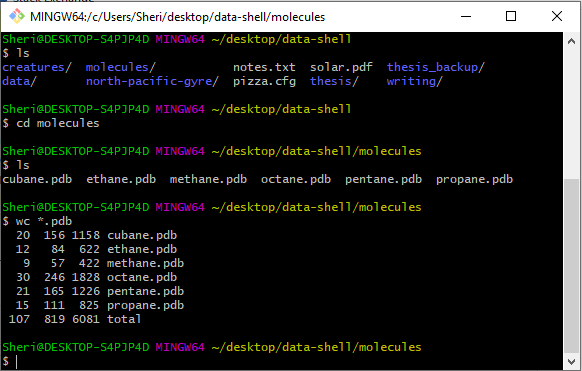
\includegraphics[width=10cm]{Images/GitBash_029.PNG}

Next we apply the filer -l to the command. I am able to do this quickly by using the up arrow to retrieve my previously entered command, and add the -l filter, instead of typing the whole string.

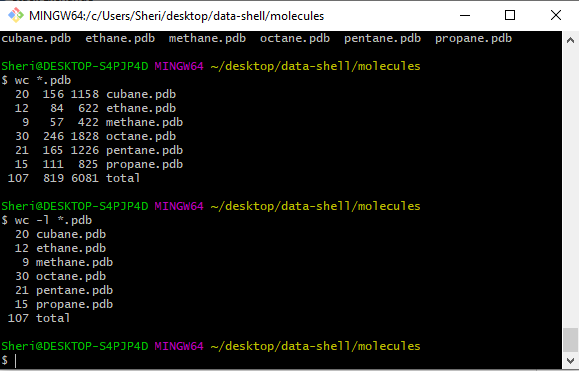
\includegraphics[width=10cm]{Images/GitBash_030.PNG}

We are then able to use the \textgreater{} symbol to redirect the result. Instead of displaying it, it will create a file, which you need to specify the name of.

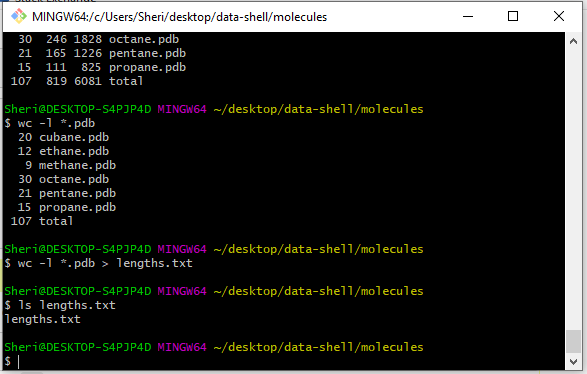
\includegraphics[width=10cm]{Images/GitBash_031.PNG}

Now we can use the sort command on the file we just created. The exercise also asked to use the -n filter to sort the output numerically. However it appears that GitBash automatically sorts numerically in ascending order. 

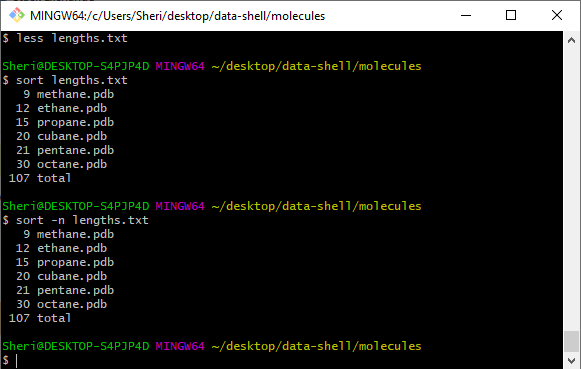
\includegraphics[width=10cm]{Images/GitBash_032.PNG}


Then we can combine this with previous commands to create a new file of the sorted data. We can also use the command, head, to return the heading, or the top rows, according to what we specify.

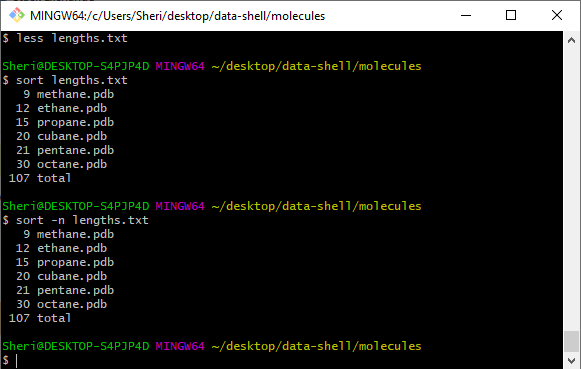
\includegraphics[width=10cm]{Images/GitBash_032.PNG}

There is advice to not try to redirecting the output onto the file that is being worked on. So I tested this. 

This is my lengths.txt file before any changes.

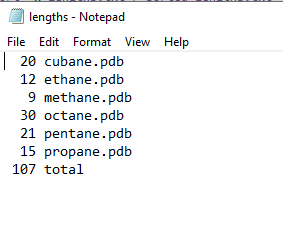
\includegraphics[width=8cm]{Images/GitBash_034a.PNG}

This is the command I ran.

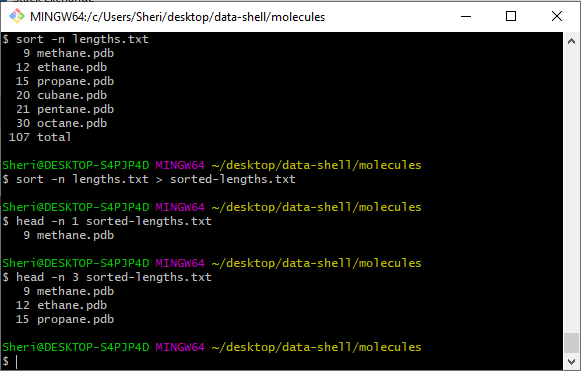
\includegraphics[width=10cm]{Images/GitBash_033.PNG}

This is how the file appeared after this.

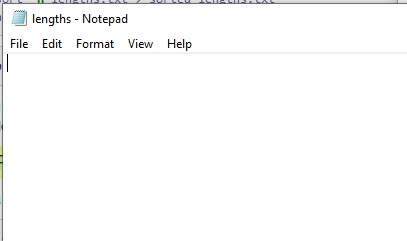
\includegraphics[width=8cm]{Images/GitBash_034.PNG}

The file was empty, the data inside it had been lost. 

\textbf{Using \textgreater{} \textgreater{}}

Using one \textgreater{} sends the output data to a file. \textgreater{}\textgreater{} works slightly differently.

To show this, I followed the exercise and entered the following commands:

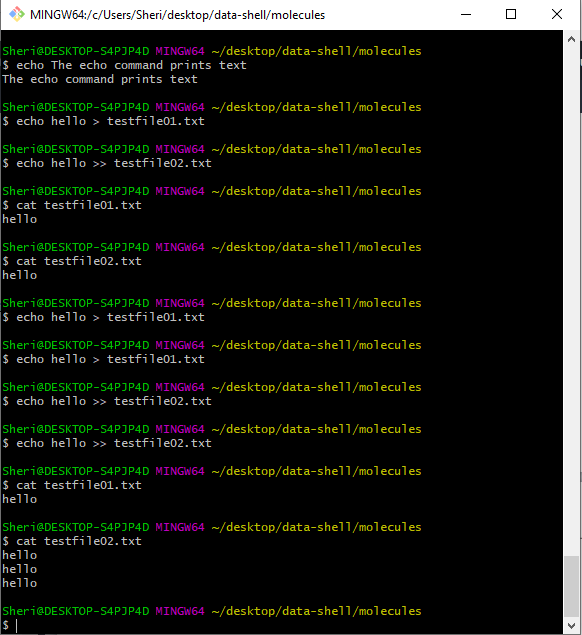
\includegraphics[width=10cm]{Images/GitBash_035.PNG}

This shows that as I entered the commands three times, the use of the \textgreater{} would overwrite the file contents, while the \textgreater{}\textgreater{} would add the new information to the existing file.

Using the | symbol, called pipe, we can combine a number of commands in sequence. 

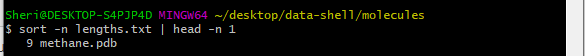
\includegraphics[width=10cm]{Images/GitBash_036.PNG}

We can combine more than two. 

Thinking through the sequence of operations is important. In the last command here, we needed to find the 3 files with the least number of lines in this directory. 

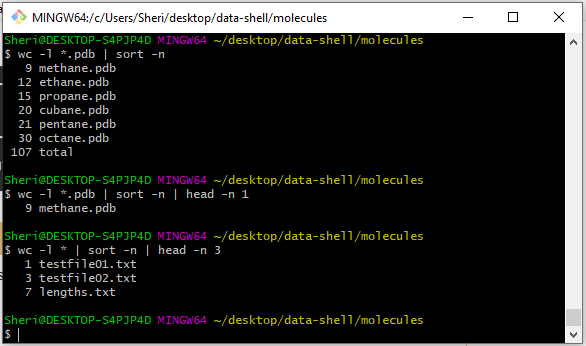
\includegraphics[width=10cm]{Images/GitBash_037.PNG}

We can validate this is correct as there is only a small number of files at this stage using ls - but it is best to be certain of the logic of the string, especially as the data sets get larger.

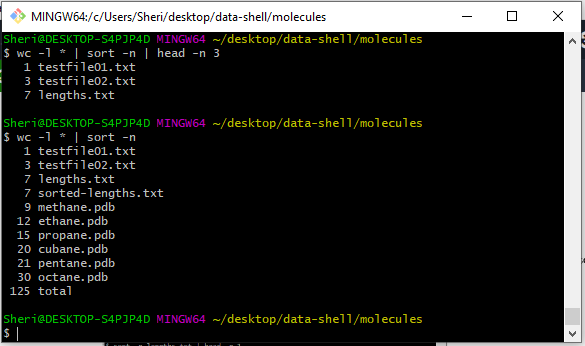
\includegraphics[width=10cm]{Images/GitBash_038.PNG}

\textbf{Pipe Reading}
In the pipe reading exercise - we must read the commands, and figure out what happens, to what data in each step.

I found this easiest when I segmented each step - and focused on the fact that the output of one command became the input for the next. 

I believe I will end up with the rows of data ending, rabbit, deer, raccoon. 

These are the strings I followed to check my thinking and outcome. 

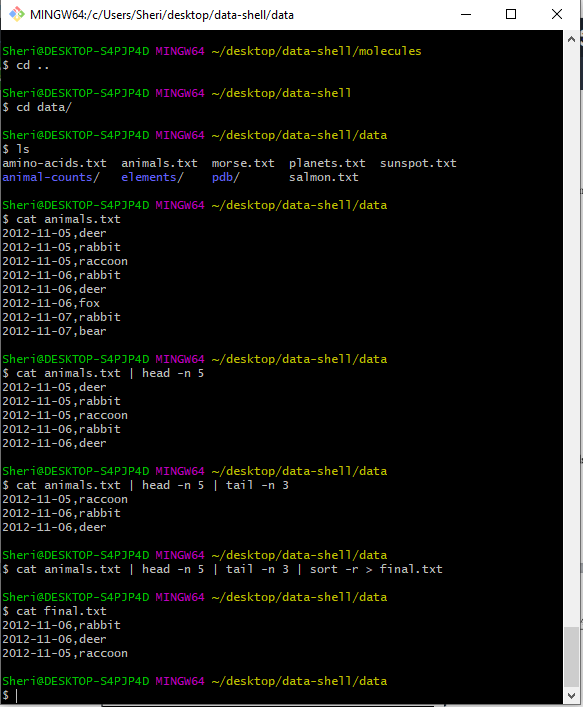
\includegraphics[width=10cm]{Images/GitBash_039.PNG}

\textbf{Pipe Construction}
In the pipe construction, we are shown the commands that will extract/isolate parts of the data we refer to. 
We then are asked to formulate a string to achieve creating a list of the unique animals listed in the file animals.txt

This is my working:

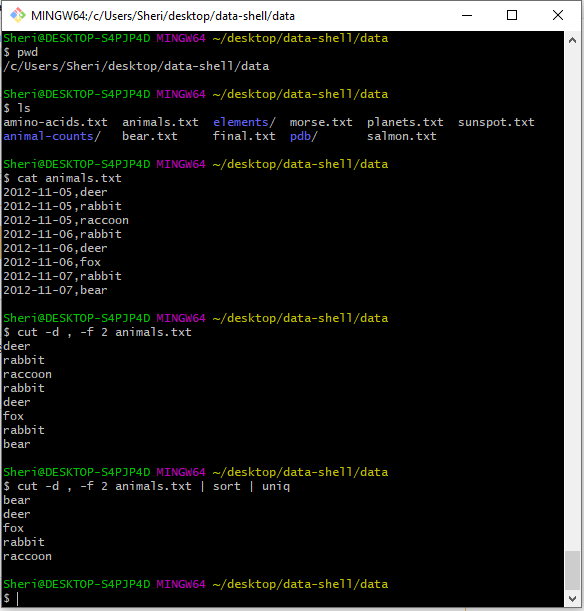
\includegraphics[width=10cm]{Images/GitBash_040.PNG}

\textbf{Which Pipe Exercise}
In this exercise we are asked to identify with string of commands will output the data we want - that being a list f the unique animals in a file, and the count of how often each appeared in the list. 

This is my working to determine option 4 was correct:

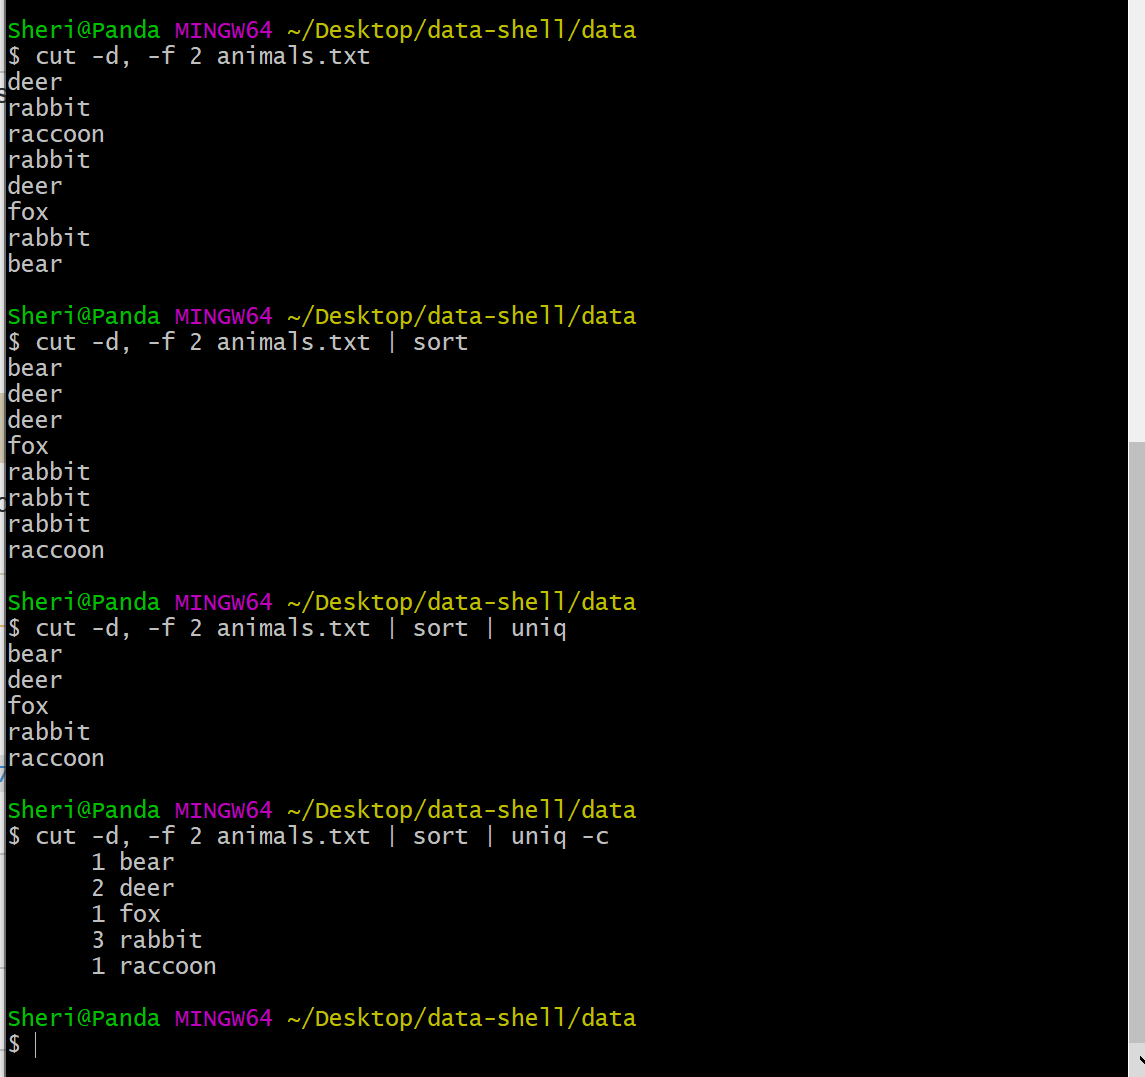
\includegraphics[width=10cm]{Images/GitBash_041.PNG}

\textbf{Wildcard Expressions}

An additional syntax we have learned is using square brackets. This works with the wildcard function to add another variable. 

In this example we want to find files ending in both a and b, but exclude files ending in z. 

So the square brackets work to offer a and b in the same string command as limiting but separate options.

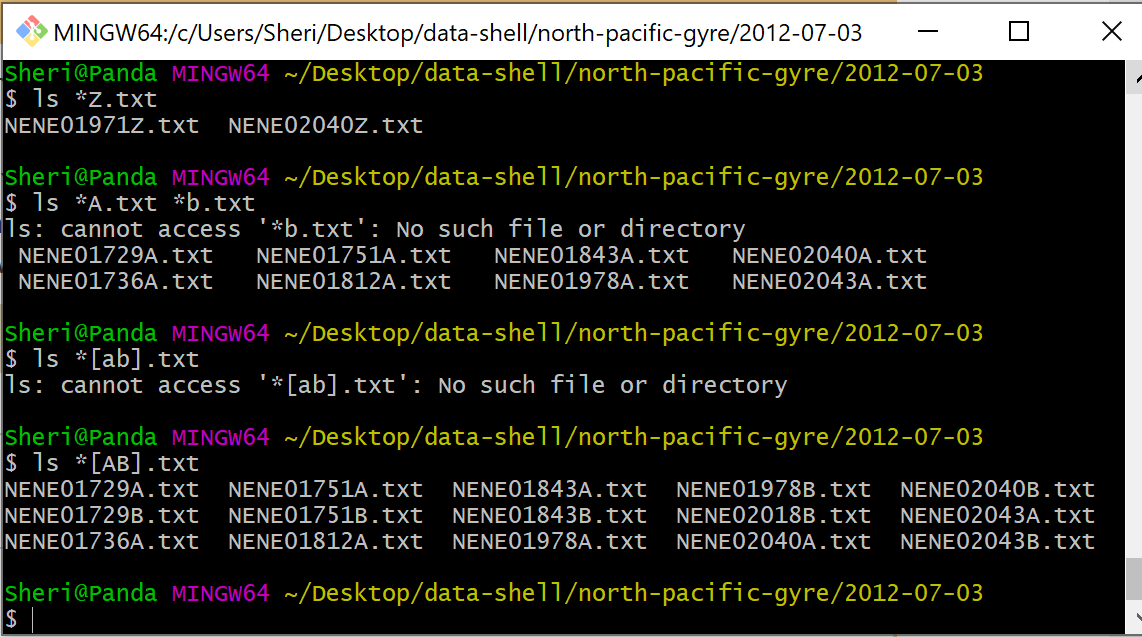
\includegraphics[width=10cm]{Images/GitBash_042.PNG}

\subsection{Loops}
Loops are a programming construct which allow us to repeat a command or set of commands for each item in a list. As such they are key to productivity improvements through automation. Similar to wildcards and tab completion, using loops also reduces the amount of typing required (and hence reduces the number of typing mistakes).

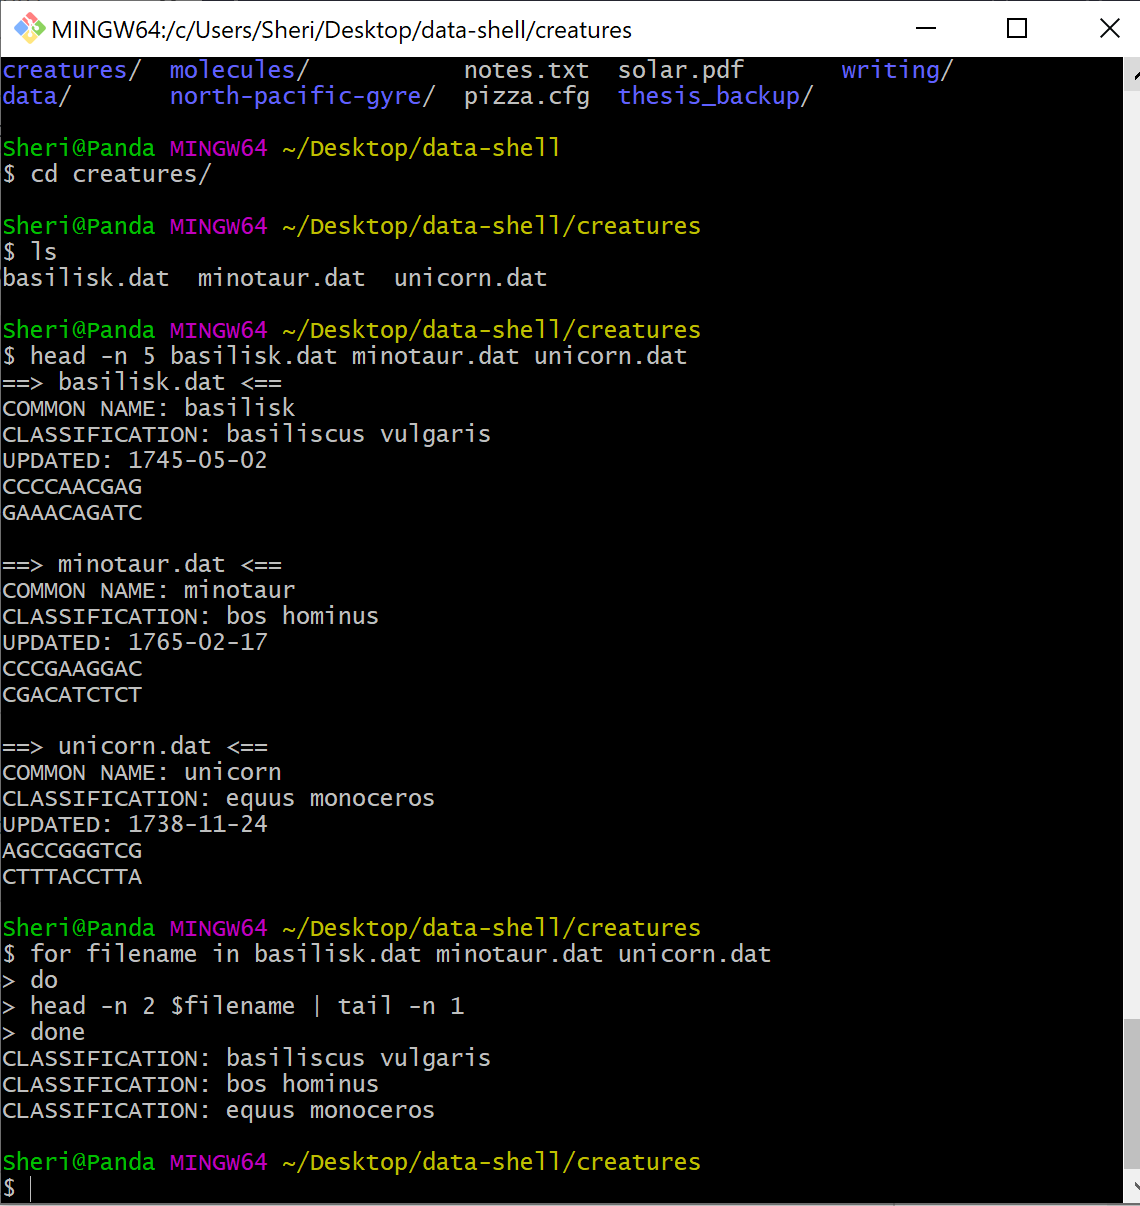
\includegraphics[width=10cm]{Images/GitBash_043.PNG}

The shell recognises we are constructing a loop, and prompts with the \textgreater{} symbol.

When the shell sees the keyword for, it knows to repeat a command (or group of commands) once for each item in a list. Each time the loop runs (called an iteration), an item in the list is assigned in sequence to the variable, and the commands inside the loop are executed, before moving on to the next item in the list. Inside the loop, we call for the variable’s value by putting \$ in front of it. The \$ tells the shell interpreter to treat the variable as a variable name and substitute its value in its place, rather than treat it as text or an external command.

\textbf{Notes on  greater than and dollar sign in Shell}
\label{Error: Notes on  greater than and dollar sign in Shell}
Here we see > being used a shell prompt, whereas > is also used to redirect output. Similarly, \$ is used as a shell prompt, but, as we saw earlier, it is also used to ask the shell to get the value of a variable.

If the shell prints > or \$ then it expects you to type something, and the symbol is a prompt.

If you type > or \$ yourself, it is an instruction from you that the shell should redirect output or get the value of a variable.


\textbf{Variables in Loops}

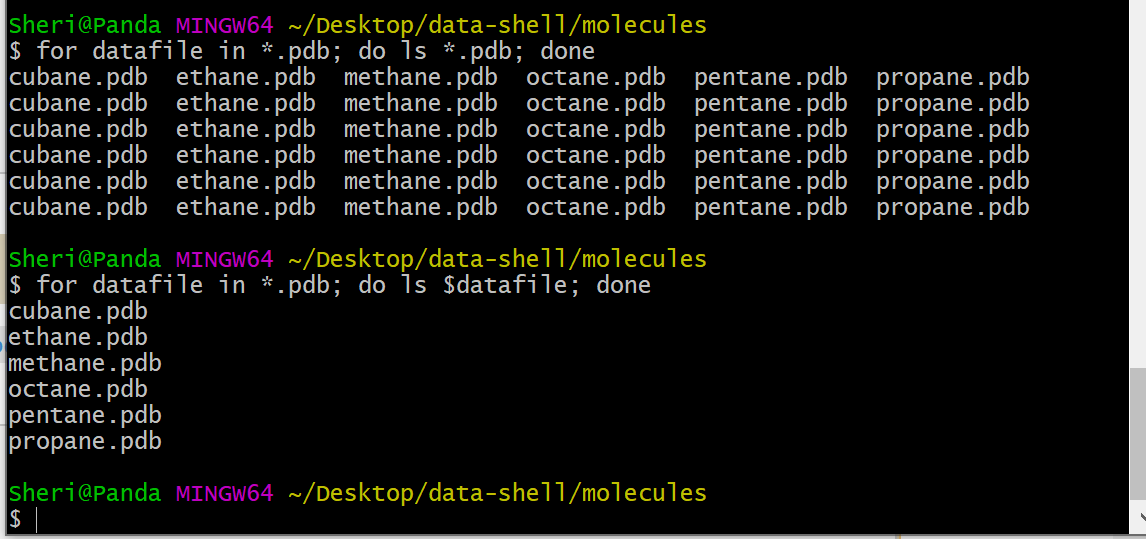
\includegraphics[width=10cm]{Images/GitBash_044.PNG}

The first code block gives the same output on each iteration through the loop. Bash expands the wildcard *.pdb within the loop body (as well as before the loop starts) to match all files ending in .pdb and then lists them using ls. 

\textbf{Limiting sets of files}

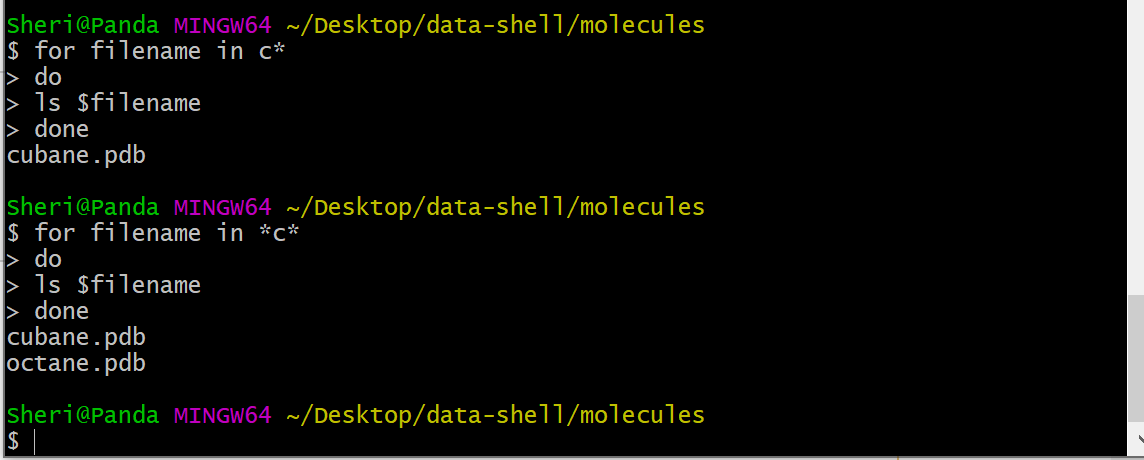
\includegraphics[width=10cm]{Images/GitBash_045.PNG}

In the second part of this exercise the solution indicates that I would have only received one file, octane.pdb as a result. However in GitBash I received both cubane.pdb and octane.pdb as a result.

\textbf{Saving a file in a loop}
\label{Error: Saving file in a loop}

When trying to run the following command loop to include outputting a file, i encountered some difficulty

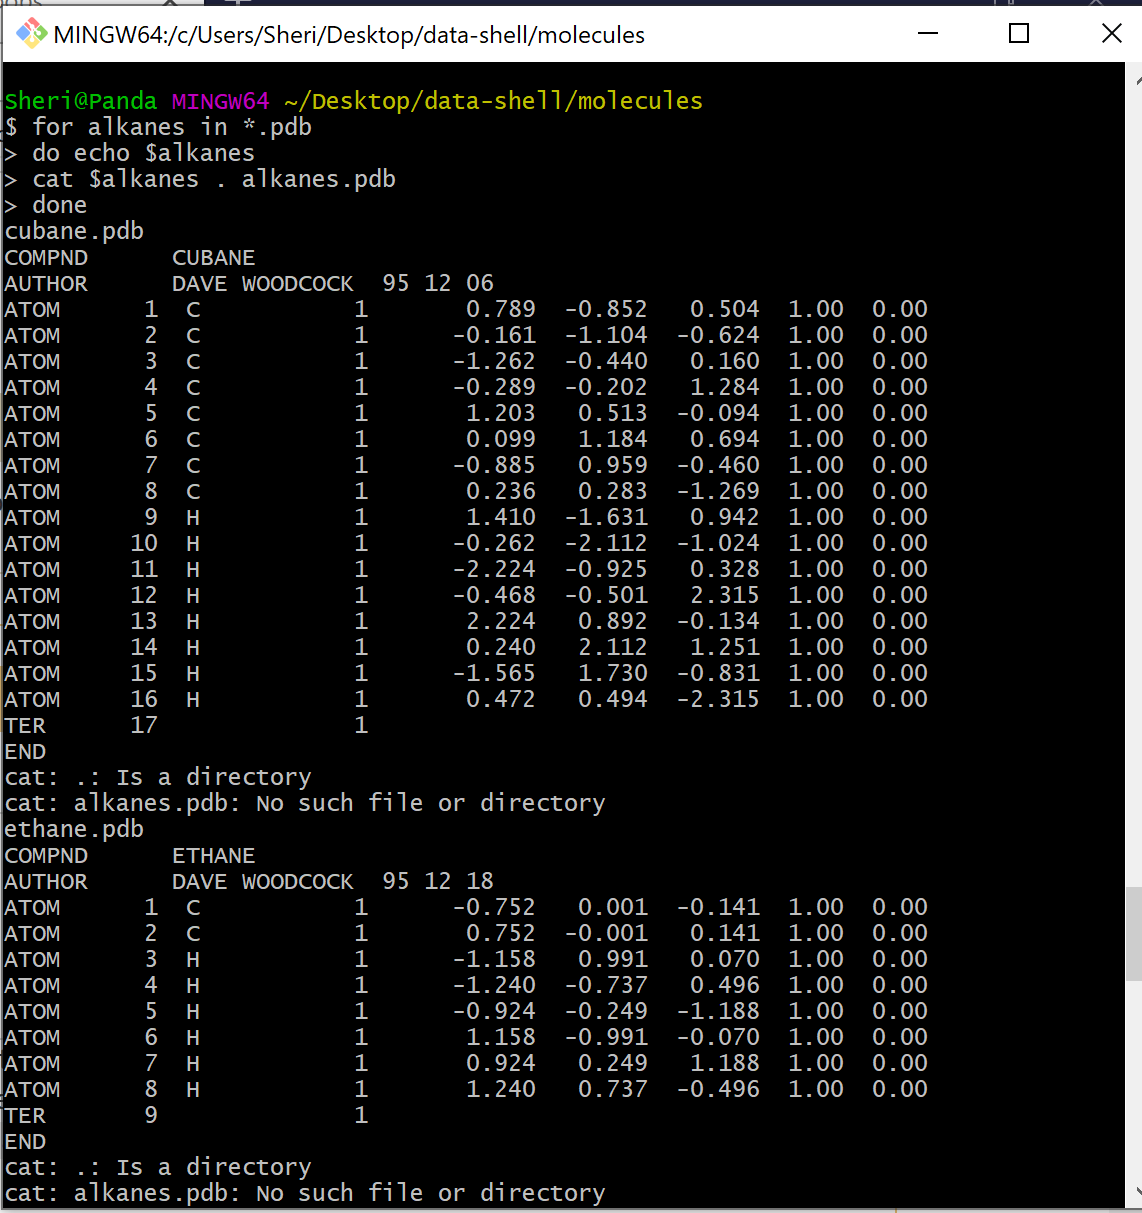
\includegraphics[width=10cm]{Images/GitBash_046.PNG}

this error occured for every time the shell tried to write to a file. The file did not exist, and so it couldn't write to the file, and it didnt create it.
it also said cat : .: is a directory

\begin{verbatim}
$  for alkanes in *.pdb
>do
>echo $alkanes
>cat $alkanes > alkanes.pdb
>done
\end{verbatim}

NB - in screenshot I can see that the entered code doesn't reflect what I had intended, and the cat: . : is not a directory error showed this.
when correcting this oversight - the code ran, but like the exercise outlined the contents of the file is the same as the finale propane file in the sequence.

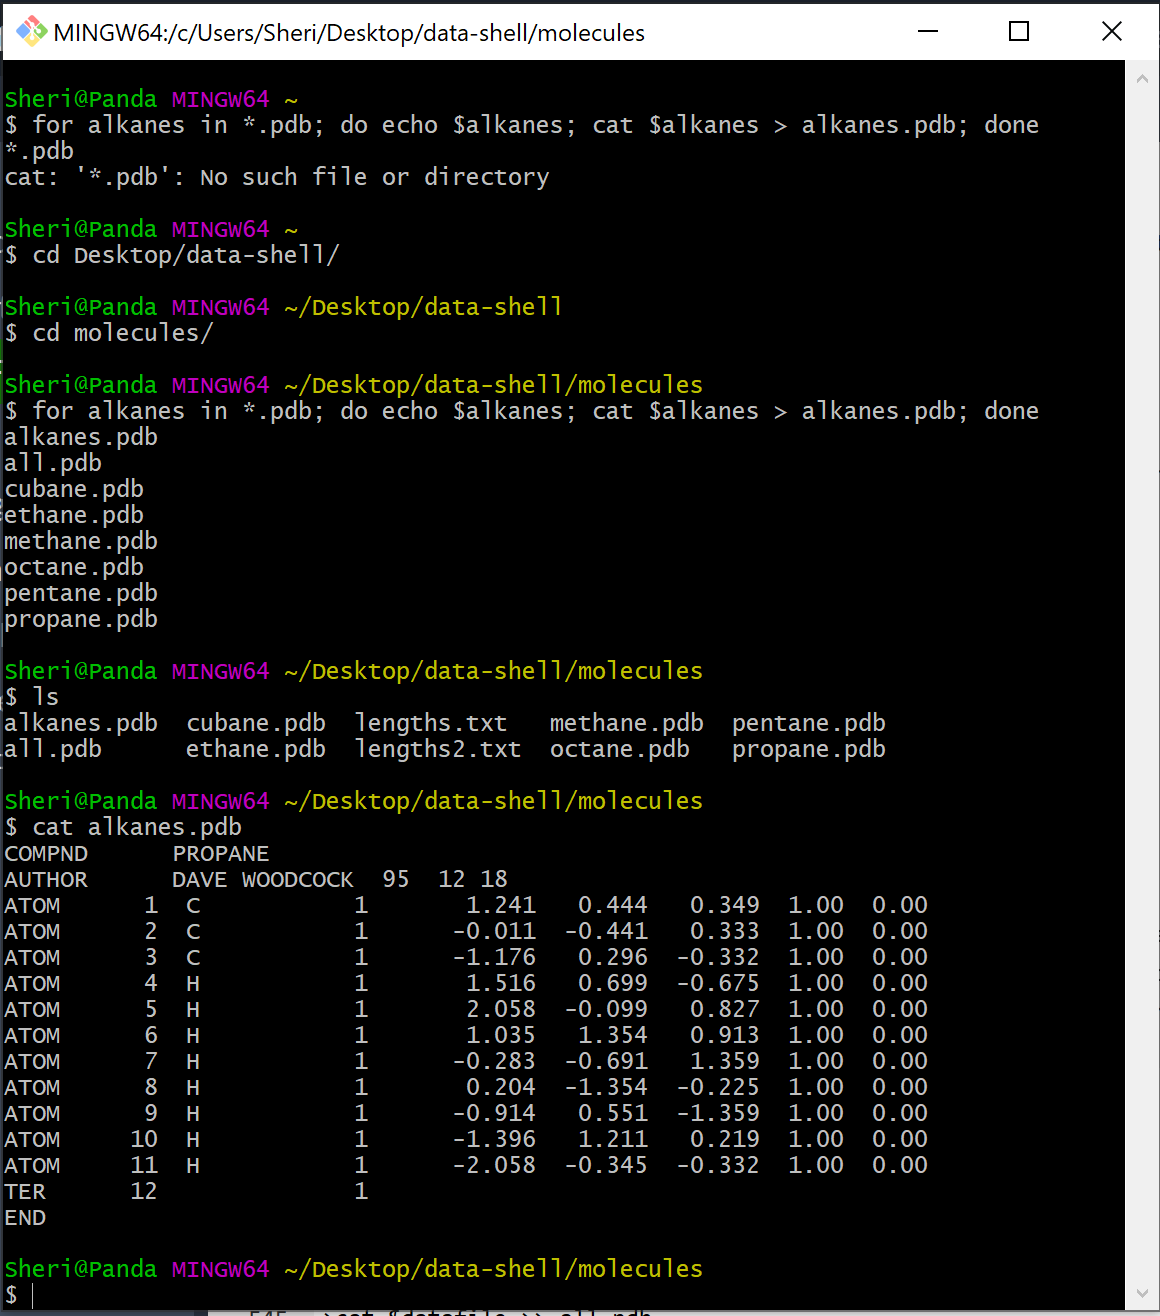
\includegraphics[width=10cm]{Images/GitBash_048.PNG}

However when I ran the following:

\begin{verbatim}
$for datafile in *.pdb
>do
>cat $datafile >> all.pdb
>done
\end{verbatim}

it worked, and cat command showed the file as intended.

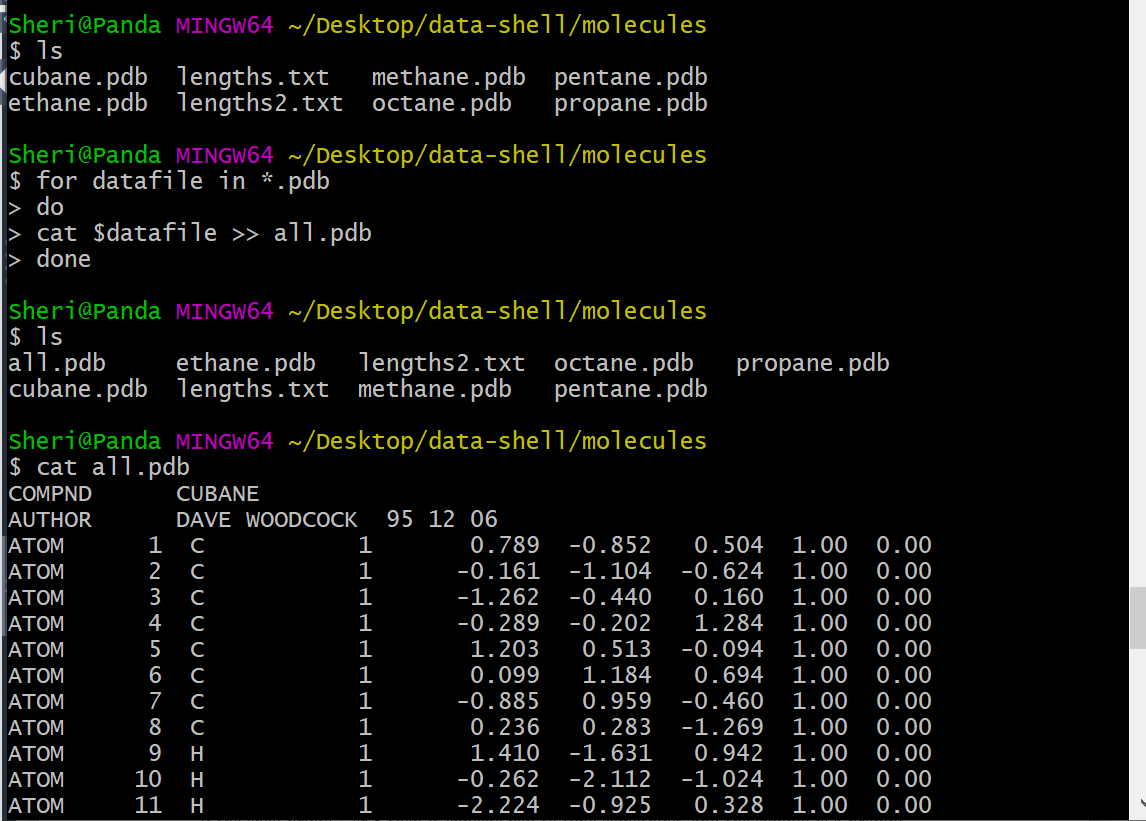
\includegraphics[width=10cm]{Images/GitBash_047.PNG}

\textbf{Spaces in Names}

Spaces are used to separate the elements of the list that we are going to loop over. If one of those elements contains a space character, we need to surround it with quotes, and do the same thing to our loop variable.

It is simpler to avoid using spaces (or other special characters) in filenames.

\textbf{Using Loops to Copy/Backup Files}

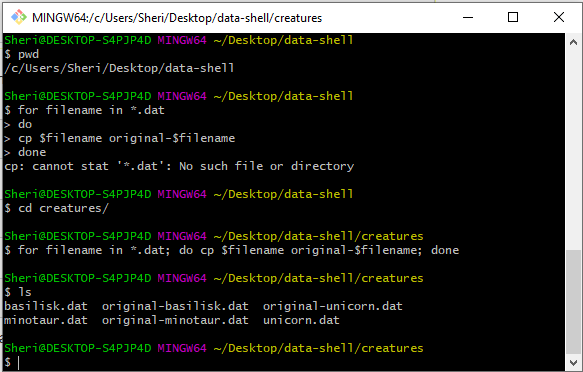
\includegraphics[width=10cm]{Images/GitBash_049.PNG}

Since the cp command does not normally produce any output, it’s hard to check that the loop is doing the correct thing. However, we learned earlier how to print strings using echo, and we can modify the loop to use echo to print our commands without actually executing them. As such we can check what commands would be run in the unmodified loop.

\textbf{Doing a dry run, using Echo command}

A loop is a way to do many things at once — or to make many mistakes at once if it does the wrong thing. One way to check what a loop would do is to echo the commands it would run instead of actually running them.

In attempting this I was worried about it executing the command and duplicating my previous work - but I realise that this is not what the echo command does in this instance - it does show the result of the loop on the screen - ``printed'' but not executed. 

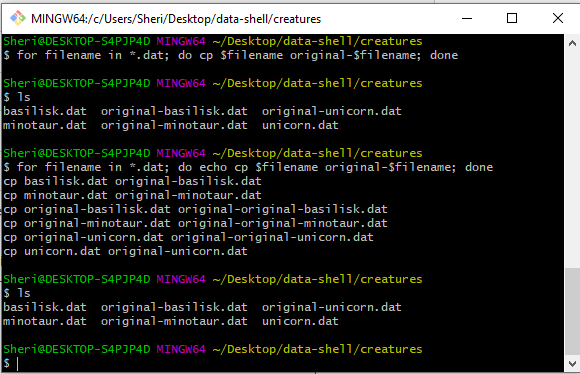
\includegraphics[width=10cm]{Images/GitBash_050.PNG}


I was able to confirm this by checking the folder after running the echo loop. 

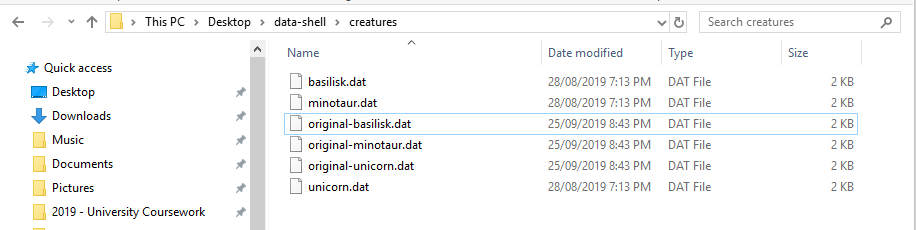
\includegraphics[width=12cm]{Images/GitBash_051.PNG}

\textbf{Nested Loop}

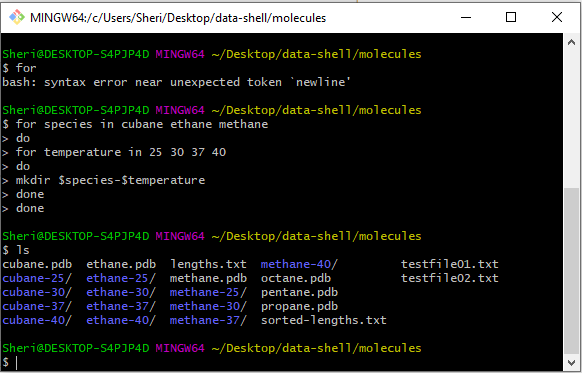
\includegraphics[width=10cm]{Images/GitBash_052.PNG}

We have a nested loop, i.e. contained within another loop, so for each species in the outer loop, the inner loop (the nested loop) iterates over the list of temperatures, and creates a new directory for each combination.

\subsection{Shell Scripts}

Creating shell scripts in a file, with the file type .sh.
Use the nano command to create a file and enter the text in the file as head -n 15 octane.pdb | tail -n 5

\includegraphics[width=10cm]{Images/GitBash_053.PNG}

We usually call programs like Microsoft Word or LibreOffice Writer “text editors”, but we need to be a bit more careful when it comes to programming. By default, Microsoft Word uses .docx files to store not only text, but also formatting information about fonts, headings, and so on. This extra information isn’t stored as characters, and doesn’t mean anything to tools like head: they expect input files to contain nothing but the letters, digits, and punctuation on a standard computer keyboard. When editing programs, therefore, you must either use a plain text editor, or be careful to save files as plain text.

\textbf{Using the shell to create a run a shell file to complete a task:}
\label{Error: Changing a shell file}

\includegraphics[width=10cm]{Images/GitBash_054.PNG}

When I edited the middle.sh file in the first instance, I forgot to delete put the octane.pdb filename, and so had an error when I tried to run the shell as an per the instructions. 
So I was able to amend the file, and run it with the expected result.

\includegraphics[width=10cm]{Images/GitBash_055.PNG}

For the same reason that we put the loop variable inside double-quotes, in case the filename happens to contain any spaces, we surround \$1 with double-quotes.

\includegraphics[width=10cm]{Images/GitBash_056.PNG}

\includegraphics[width=10cm]{Images/GitBash_057.PNG}

To make it easier for ourselves or someone else to know what the string is does, and how to use it we can add comments in the file.

\includegraphics[width=10cm]{Images/GitBash_058.PNG}

A comment starts with a \# character and runs to the end of the line.

The only caveat is that each time you modify the script, you should check that the comment is still accurate: an explanation that sends the reader in the wrong direction is worse than none at all.


\textbf{Listing Unique species exercise}

\includegraphics[width=10cm]{Images/GitBash_059.PNG}

\textbf{typos in Shell files}
\label{Error: Typos in Shell files}

While there was a typo error in one part of the shell script - it continued to attempt to run the remainder of the script. So I knew there was an error in one line only that affected the output.

\includegraphics[width=10cm]{Images/GitBash_060.PNG}

Once the typo was corrected - the shell script ran as expected. 

\textbf{Using History command to record/save a useful string}

When you run a number of commands and want to save them, the history command can do this. History will show a list of recent commands - which can be added to the tail command in a pipe to output the commands you want to save. This can be output to a file - which with some clean up and added comments can be a useful shell file that can be reused later.

Note that commands are saved in the history before being run. This is helpful when a command causes an error or a crash - as it is then possible to know what caused the issue. When using history then, make sure you allow for the most recent item to be the history command that you run to create that same list ( and adjust the tail argument accordingly).



\subsection{Finding Things}

\textbf{Using GREP to find things}
 
 ``grep'' is a contraction of ‘global/regular expression/print’, a common sequence of operations in early Unix text editors. It is also the name of a very useful command-line program.
 
The command grep finds and prints lines in files that match a pattern. 
This is case sensitive, and it is useful to include the searched for item in quotation marks, even if only a single word - as it aids how we think about using grep.

Using grep to find all instances of the sequence ``not'', a``the'', and ``The.''


\includegraphics[width=10cm]{Images/GitBash_061.PNG}

Beginning to use arguments to refine/adjust the grep search

\includegraphics[width=10cm]{Images/GitBash_062.PNG}

\includegraphics[width=10cm]{Images/GitBash_063.PNG}

\includegraphics[width=10cm]{Images/GitBash_064.PNG}


Using grep to detimine which string will produce a single line as a result:

\includegraphics[width=10cm]{Images/GitBash_065.PNG}

Using the -w argument is what will achieve this - as this searches for complete words, not the sequence as part of a word.

\textbf{Wildcards}

grep’s real power doesn’t come from its options, though; it comes from the fact that patterns can include wildcards. (The technical name for these is regular expressions, which is what the ‘re’ in ‘grep’ stands for.)

We use the -E option and put the pattern in quotes to prevent the shell from trying to interpret it. (If the pattern contained a *, for example, the shell would try to expand it before running grep.) The \^ in the pattern anchors the match to the start of the line. The . matches a single character (just like ? in the shell), while the o matches an actual `o'.

\includegraphics[width=10cm]{Images/GitBash_066.PNG}

\textbf{Listing vs. Finding}

ls and find can be made to do similar things given the right options, but under normal circumstances, ls lists everything it can, while find searches for things with certain properties and shows them.

The find command can be given several other criteria known as “tests” to locate files with specific attributes, such as creation time, size, permissions, or ownership. 


\pagebreak

\section{OpenRefine for Social Sciences}


\subsection{Set Up}

OpenRefine is downloaded from www.openrefine.org

It requires a java plug in, and the download for this is prompted during installation if necessary.

The tool will run start up in a window, and then open the working tool in a browser window where you will work on your data.

\subsection{Introduction}

OpenRefine is an open-source and free tool for working with messy data. It enables cleaning up said data, and recording how this is done - which is useful for academics in providing data provenance with their studies.


\subsection{Working with OpenRefine}

When you work on a file in OpenRefine it is called a project. OpenRefine also doesn't make changes to your original raw data. Which is useful for data provenance and also rectifying any mistakes or data corruption.

To create a new project you import your data by browsing files on your computer. OpenRefine is able to work with a variety of file formats, and this should be specified during the import.

The Parse next field indicates how many rows of the data contains the column headings, or other information that isn't the data itself - eg, headings, metadata notes.

To then progress to working on your file click the create project button. 

\textbf{Facets}

Facets are a key part of working in OpenRefine. 


Using a text facet we can see that the data in the `villages' column has some discrepancies.

We can also see that the facet shows the text, and the number of time/rows it occurs in. 

We could correct these discrepancies using the `edit' function within the facet - and the changes could be applied to all similar values in the data range (the village column). 

There are other ways to make these changes though.

\textbf{Numeric data in OpenRefine}
\label{Error: Numeric data in OpenRefine}

NB: all data is imported into OpenRefine as if it were text - and so when wanting to work with data numerically, we must `transform' the data type from text to numeric.

We discovered this is trying to facet the interview date column numerically, and the result was that the column did not contain numerical data.

I had originally thought that this a reflected in the data being presented with the month appearing as letters, but that was a misinterpretation, and reflective of how the data was formatted, not the data the cell contained. 

\textbf{Clustering}

To fix the discrepancies in the `villages' column, we can use the clustering function in the facet we created.

When we click `cluster' a window opens, and various methods of clustering the data points, and their outcome are listed. There are also `keying functions' which can be adjusted for different results.

We can chose any we would like to adopt, and redo this process numerous times to further refine the data.

Though there are some data points that cannot be refined this way, because they are not similar enough to be certain of the accuracy of the change. For example in the `villages' column, there is a field containing `49,' which cannot be merged with any of the other names without more information.

In this case as well, the clustering did not merge all parts that we believe should have been, like  `Chirdozo' with `Chirodzo'. As humans we can see that this is likely a typo, and so we can use the edit within the facet to make this change manually.

\textbf{Transforming Data}

In the column `items owned' the information is separated by numerous characters, ;, ', [, and ].

These create difficulties in faceting the column to something useful, so we must remove some of the extraneous characters. 

Using the `transform' function, we can apply a GREL expression to execute a change within this data, as using the cluster function is not appropriate.

the GREL strings we use to clean this column are:
\begin{itemize}
    \item value.replace("[", "")
    \item value.replace("]", "")
    \item value.replace("'", "")
    \item value.replace(" ", "")
\end{itemize}

These can all be combined into one string, with multiple actions. eg: value.replace("'","").replace("[","").replace("]","").replace(" ","") 

We end up with the information separated in the column only by ;

We can then facet the column, but using a custom facet, to indicate the information is separated by ; and view the information in a way that is useful. This must be entered in the Expression field of the custom facet window as value.split(";")

This tells us that the two most commonly owned items are mobile phones and radios, and the two least commonly owned are cars and computers.

We can apply this same process to the months without food column, and surmise that the month most commonly identified by the respondents as being without food is November.

We can `reuse' previous GREL expressions in the transform window by going to the history tab. This is useful for applying the same cleanup to other columns.

\textbf{Undo and Redo}

It is possible to undo/redo multiple steps in OpenRefine. The undo/redo button also acts as a record of all actions applied to the project, and acts more like a menu than an instantaneous button.

We are able to then undo multiple steps, and OpenRefine will enact that visually for us to check before confirming/continuing. We are then able to redo multiple actions in the same way. 

I can see this being useful if a mistake is made in a step but not noticed immediately, and so you could backtrack through your actions to discover which step caused the error and correct from that point specifically.

\textbf{Trim Leading and Trailing Whitespace}

There are a number of `common' transformations that OpenRefine allows to apply quickly and easily.

When we facet the wall type column, a field is separated even though it looks like it should be grouped with muddaub. This is because some of the cell entries contain an extra space after the word, which the computer notes, but the human eye doesn't necessarily see. 

Using the common transform function to trim leading and trailing whitespace, we can use a previously established function to resolve this and further refine our project.

\subsection{Filtering and Sorting with OpenRefine}

\textbf{Filtering}
\textbf{Error: Filters doesn't automatically summon the text facet box}
\label{Error: Filter doesn't automatically summon the text facet box}

In addition to facets, filtering is a useful tool to work on subsets of data within your project.

Then course instructions imply that applying the text filter will also automatically cause the text facet box to appear on the left of the screen. I found that this wasn't the case in my experience, the text filter acted similar to a filter in excel, in that when applied it  only showed the rows with data that matched the filter conditions. 

However when I apply the facet, the text filter is automatically applied to the facet, and vice versa.

After applying a text facet to the column `respondent roof type', we can further filter the data.

We find that when filtering by `mabat', we have two data results that match the filter. 

At the top left of the screen it confirms the filter in place, and highlights then number of rows selected. in this case we are working within 58 rows of a total of 131. 

There is also the option to visualise more or less rows in the project - but this doesn't change the amount of rows selected through the filter. 

Facets are applied in order, and subsequent facets will apply to the data filtered previously, but not to the excluded data.

The refine the search we could filter using more letters. Or select one of the text facet results. and use the inlcude/exclude buttons.

Ensure that when moving on to other tasks, you remove facets to ensure you are again  working with your full data, as in all 131 rows of data. So for our next steps we must remove these facets, and return to working with the full data set for the next part.


\textbf{Sort}

Similar to filtering, in the drop down menu from a column heading we can also sort the rows.

We apply a sort to the column `gps altitude.' This reveals a number of cells with zero entered, and the next is a number over 600. We are then able to surmise that the zero points are most likely due to the information not being recorded - in the case of the gps signal being lost when the data was collected. 

Once a sort is applied to a column, the drop down will then show the sort item with an arrow next to it, leading to more options, like reverse and remove sort, this also indicates that the column has already been sorted. 

\textbf{Sorting by multiple columns}

The sort function can be applied to multiple columns, and subsequent sorts work withing the order of the previously applied sort.

We can use this to find out the correct village for the entry `49' in the village column.

Using the edit column to move the village column to the end, we can compare the village data to gps information. Sorting to group the gps information seems to imply that `49' could be `Chirodzo', but it is not conclusive as other villages have very similar gps coordinates.

By moving the village column back to the beginning, and comparing to the interview date instead, we can see that the only village interviewed on the same date as entry `49' is in fact Chirodzo, so we can apply this change confident in our reasoning to its accuracy.

\textbf{Error: Removing ALL sorts before attempting next task}
\label{Error: Removing ALL sorts before attempting next task}

I found that i had issues after moving the village column back to the beginning and trying to compare then interview dates. this was because I hadn't completely removed all the sorts on the gps columns. 

I went back and removed the sorts, but I could have also used the Undo/Redo record to see which one had not been removed.

\subsection{Examining Numbers in OpenRefine}

Data is automatically assumed to be text in OpenRefine, unless otherwise specified. Use the transform function to change the way data in a column behaves, eg from text to number.

\textbf{Numeric Facet}

After changing the `years farm' column to number, we can run  a numeric facet on the column. The information appears differently to a text facet - presenting as a numeric range that can be filtered by adjusting the highlighted range.

If a text cell is included in a numeric sort, some more check boxes appear at the bottom of the facet - allowing the option in include or exclude non-numeric data. By checking and unchecking these boxes, it changes the rows that are selected and appear on the screen.

\subsection{Using Scripts}

It is possible to save your OpenRefine as a script. 

In the Undo/Redo tab, you can extract this. This generates a body of text that can be copied and placed in a text editor (Not Word) and saved as a csv file. 

It is possible to filter the actions that you want to include in the extracted data using the checkboxes next to the tasks in the list.

Then you can take this list of operations and apply it to a new project. In the Undo/Redo tab, we can click the apply button, and copy and paste the contents of our created csv file, and then choosing the perform operations button will apply that work to the current project.

\subsection{Exporting and Saving Data from Open Refine}

SO until now, we have been working on lour data in OpenRefine, but it is locked into that space. The saved raw file is unchanged. So we need to export our refined/worked data.

\textbf{Saving}

OpenRefine saves your work continuously, enabling you to reopen your project and continue work without excessive steps.

\textbf{Exporting}
\label{Exporting}

The instructions for exporting the project from OpenRefine run as follows: 
\begin{itemize}
    \item Click the Export button in the top right and select Export project.
    \item A tar.gz file will download to your default Download directory. Depending on your browser you may have to confirm that you want to save the file. The tar.gz extension tells you that this is a compressed file. The downloaded tar.gz file is actually a folder of files which have been compressed. Linux and Mac machines will have software installed to automatically expand this type of file when you double-click on it. For Windows based machines you may have to install a utility like ‘7-zip’ in order to expand the file and see the files in the folder.
    \item After you have expanded the file look at the files that appear in this folder. What files are here? What information do you think these files contain?
\end{itemize}

The exercise solutions states the following
\begin{itemize}
    \item  a history folder which contains a collection of zip files. Each of these files itself contains a change.txt file. These change.txt files are the records of each individual transformation that you did to your data.
    \item a data.zip file. When expanded, this zip file includes a file called data.txt which is a copy of your raw data. You may also see other files.
\end{itemize}

However in my experience the zipped file has a gz file extension, and as a windows 10 user, I was unable to unzip this file to see it's contents. The lesson suggested downloading a program called 7-zip, but I was unable to find this online. 

I was able to import the .gz file back to OpenRefine though and open the data and the operations history.

I was able to export the data as a csv and open it in excel. however this form doesn't preserve all the operations as well, which I believe the standard export would do.


\subsection{Other Resources in Open Refine}

As an opensource tool, there is a diverse range of information and support available for OpenRefine. 
There are numerous resources offered through www.openrefine.org but also a range of associated sites like https://github.com/scottythered/gratefuldata/wiki which has useful and interesting information about data and working with data.


\section{R for Social Sciences}
\subsection{Before we Start}

R is a programming language, while R Studio is a programming environment that utilises R language.

It allows for a series of script commands to be saved and rerun at a later time - which is useful for researchers working with an expanding data-set. 

This is a aspect of reproducible research which is beneficial for researchers. This allows new data to be treated in exactly the same way as previous data, and ensures integrity of the data processing process. 

\subsection{Requirements}

\url{https://datacarpentry.org/r-socialsci/}

\begin{itemize}
    \item Download and install R
    \item Download and install R studio
\end{itemize}

You will also need to install tidyverse in RStudio to complete the exercises.


\subsection{Setting up a new project}

To set up a new project, open R studio:

Go to:
\begin{enumerate}
    \item File
    \item New Project - A window will open
    \item Click on New Directory
    \item Enter a name for your new project - eg: DataCarpentry
    \item Click on Create Project 
\end{enumerate}

Your project has now been created.

In this project you will need to set up some folders to organise your work. Use the create.dir("folder\_name") command in the terminal to create the following folders:
\begin{itemize}
    \item data
    \item data\_output
    \item fig\_output
\end{itemize}

I ran the commands, and ended up with this in my files list:

\includegraphics[width=8cm]{Images/RStudio001.PNG}

I was also able to run the command given in the exercise to download the data file to the folder.

\includegraphics[width=8cm]{Images/RStudio002.PNG}

This is the terminal screen showing the commands to create the folders, and download the example file:

\includegraphics[width=10cm]{Images/RStudio003.PNG}


Then install the tidyverse package:

\includegraphics[width=10cm]{Images/RStudio004.PNG}

\subsection{Creating Objects in R}

What are known as objects in R are known as variables in many other programming languages. Depending on the context, object and variable can have drastically different meanings. However, in this lesson, the two words are used synonymously. 
An object is something to which I can assign a value. In the example we work through in the exercise "area\_hectare" is an object, as is "area\_acres"



\includegraphics[width=8cm]{Images/RStudio005.PNG}

This is the environment in the top right of the window, where the assigned values are displayed.

\includegraphics[width=8cm]{Images/RStudio006.PNG}

At the end of these series of exercises - the area\_acres doesn't change as we don't rerun the assignment command - which is what determines that objects value. It isn't set in a direct relationship with the value of area\_hectares.

To complete this exercise, we assign a value to length, and width, then use those values to create and assign a value to area. Then changing the values assigned to width and length, we can see that as expected the value of area doesn't change.

Assigning the initial values:

\includegraphics[width=8cm]{Images/RStudio007.PNG}

Changing the assigned values:

\includegraphics[width=8cm]{Images/RStudio009.PNG}

Showing the area value remains unchanged - unless the assignment command is rerun.

\includegraphics[width=8cm]{Images/RStudio008.PNG}


\subsection{Functions and their arguments}

Functions are “canned scripts” that automate more complicated sets of commands including operations assignments, etc. Many functions are predefined, or can be made available by importing R packages (more on that later). A function usually gets one or more inputs called arguments. Functions often (but not always) return a value. A typical example would be the function sqrt(). The input (the argument) must be a number, and the return value (in fact, the output) is the square root of that number. Executing a function (‘running it’) is called calling the function.




\subsection{Vectors and Data Types}
 vector is the most common and basic data type in R, and is pretty much the workhorse of R. A vector is composed by a series of values, which can be either numbers or characters. We can assign a series of values to a vector using the c() function. For example we can create a vector of household members for the households we’ve interviewed and assign it to a new object hh\_members:
 
\includegraphics[width=10cm]{Images/RStudio010.PNG}

Testing combined vectors and outputs:

\includegraphics[width=10cm]{Images/RStudio011.PNG}


\subsection{Subsetting Vectors}

Using indices to extract specific information from a vector value.

\includegraphics[width=8cm]{Images/RStudio012.PNG}

\subsection{Conditional Subsetting}

Using TRUE/FALSE conditions for subset filtering.

Also using == and <= and >= and < and > as refining filters.

\includegraphics[width=8cm]{Images/RStudio013.PNG}

\includegraphics[width=8cm]{Images/RStudio014.PNG}


\subsection{Missing Data}

As R was designed to analyze datasets, it includes the concept of missing data (which is uncommon in other programming languages). Missing data are represented in vectors as NA.

When doing operations on numbers, most functions will return NA if the data you are working with include missing values. This feature makes it harder to overlook the cases where you are dealing with missing data. You can add the argument na.rm=TRUE to calculate the result while ignoring the missing values.

\includegraphics[width=8cm]{Images/RStudio015.PNG}

\subsection{Starting with Data}

SAFI (Studying African Farmer-Led Irrigation) is a study looking at farming and irrigation methods in Tanzania and Mozambique. The survey data was collected through interviews conducted between November 2016 and June 2017. For this lesson, we will be using a subset of the available data. For information about the full teaching dataset used in other lessons in this workshop, see the dataset description.

We will be using a subset of the cleaned version of the dataset that was produced through cleaning in OpenRefine. Each row holds information for a single interview respondent, and the columns represent:

You are going load the data in R’s memory using the function read\_csv() from the readr package which is part of the tidyverse. So, before we can use the read\_csv() function, we need to load the package. Also, if you recall, the missing data is encoded as “NULL” in the dataset. We’ll tell it to the function, so R will automatically convert all the “NULL” entries in the dataset into NA.


\includegraphics[width=10cm]{Images/RStudio016.PNG}

Checking data set has been assigned and "read" correctly:

\includegraphics[width=10cm]{Images/RStudio017.PNG}



\subsection{Data Frames and Tibbles}

Data frames are the de facto data structure for tabular data in R, and what we use for data processing, statistics, and plotting.

A data frame is the representation of data in the format of a table where the columns are vectors that all have the same length. Because columns are vectors, each column must contain a single type of data (e.g., characters, integers, factors). For example, here is a figure depicting a data frame comprising a numeric, a character, and a logical vector.

A data frame can be created by hand, but most commonly they are generated by the functions read\_csv() or read\_table(); in other words, when importing spreadsheets from your hard drive (or the web).

A tibble is an extension of R data frames used by the tidyverse. When the data is read using read\_csv(), it is stored in an object of class tbl\_df, tbl, and data.frame. You can see the class of an object with

\includegraphics[width=8cm]{Images/RStudio018.PNG}

As a tibble, the type of data included in each column is listed in an abbreviated fashion below the column names. For instance, here key\_ID is a column of integers (abbreviated <int>), village is a column of characters (<chr>) and the interview\_date is a column in the “date and time” format (<dttm>).

\subsection{Inspecting Data Frames}

When calling a tbl\_df object (like interviews here), there is already a lot of information about our data frame being displayed such as the number of rows, the number of columns, the names of the columns, and as we just saw the class of data stored in each column. However, there are functions to extract this information from data frames. Here is a non-exhaustive list of some of these functions. Let’s try them out!

\includegraphics[width=10cm]{Images/RStudio019.PNG}

\includegraphics[width=10cm]{Images/RStudio020.PNG}

\includegraphics[width=10cm]{Images/RStudio021.PNG}

\subsection{Indexing and Subsetting Data Frames}

Our interviews data frame has rows and columns (it has 2 dimensions), if we want to extract some specific data from it, we need to specify the “coordinates” we want from it. Row numbers come first, followed by column numbers. However, note that different ways of specifying these coordinates lead to results with different classes.
    
\includegraphics[width=10cm]{Images/RStudio022.PNG}

: is a special function that creates numeric vectors of integers in increasing or decreasing order, test 1:10 and 10:1 for instance.

You can also exclude certain indices of a data frame using the “-” sign:    

\includegraphics[width=10cm]{Images/RStudio023.PNG}

\subsection{Factors}

R has a special data class, called factor, to deal with categorical data that you may encounter when creating plots or doing statistical analyses. Factors are very useful and actually contribute to making R particularly well suited to working with data. So we are going to spend a little time introducing them.

Factors represent categorical data. They are stored as integers associated with labels and they can be ordered or unordered. While factors look (and often behave) like character vectors, they are actually treated as integer vectors by R. So you need to be very careful when treating them as strings.

Once created, factors can only contain a pre-defined set of values, known as levels. By default, R always sorts levels in alphabetical order. For instance, if you have a factor with 2 levels:

\includegraphics[width=10cm]{Images/RStudio024.PNG}

In R’s memory, these factors are represented by integers (1, 2), but are more informative than integers because factors are self describing: "cement", "earth" is more descriptive than 1, and 2. Which one is “earth”? You wouldn’t be able to tell just from the integer data. Factors, on the other hand, have this information built in. It is particularly helpful when there are many levels. It also makes renaming levels easier. Let’s say we made a mistake and need to recode “cement” to “brick”.

\includegraphics[width=10cm]{Images/RStudio025.PNG}

\subsection{Converting Factors}

If you need to convert a factor to a character vector, you use as.character(x).

\includegraphics[width=10cm]{Images/RStudio026.PNG}

The last way is the recommended way - as it is consistent and reliable. 

\subsection{Renaming Factors}

When your data is stored as a factor, you can use the plot() function to get a quick glance at the number of observations represented by each factor level. Let’s extract the memb\_assoc column from our data frame, convert it into a factor, and use it to look at the number of interview respondents who were or were not members of an irrigation association:

\includegraphics[width=10cm]{Images/RStudio027.PNG}

\includegraphics[width=10cm]{Images/RStudio028.PNG}

\includegraphics[width=10cm]{Images/RStudio029.PNG}

\includegraphics[width=10cm]{Images/RStudio030.PNG}

Exercise Outcome:

\includegraphics[width=10cm]{Images/RStudio031.PNG}

\includegraphics[width=10cm]{Images/RStudio032.PNG}


\subsection{Formatting Dates}

One of the most common issues that new (and experienced!) R users have is converting date and time information into a variable that is appropriate and usable during analyses. As a reminder from earlier in this lesson, the best practice for dealing with date data is to ensure that each component of your date is stored as a separate variable. In our dataset, we have a column interview\_date which contains information about the year, month, and day that the interview was conducted. Let’s convert those dates into three separate columns.


\includegraphics[width=10cm]{Images/RStudio033.PNG}

\subsection{Data Manipulation using dplyr and tidyr}

dplyr is a package for making tabular data manipulation easier by using a limited set of functions that can be combined to extract and summarize insights from your data. It pairs nicely with tidyr which enables you to swiftly convert between different data formats (long vs. wide) for plotting and analysis.

Similarly to readr, dplyr and tidyr are also part of the tidyverse. These packages were loaded in R’s memory when we called library(tidyverse) earlier.

\subsection{Selecting columns and filtering rows}

To select columns of a data frame, use select(). The first argument to this function is the data frame (interviews), and the subsequent arguments are the columns to keep.

To choose rows based on a specific criteria, use filter():

\includegraphics[width=10cm]{Images/RStudio034.PNG}


\subsection{Pipes}

What if you want to select and filter at the same time? There are three ways to do this: use intermediate steps, nested functions, or pipes.

With intermediate steps, you create a temporary data frame and use that as input to the next function, like this:

\includegraphics[width=10cm]{Images/RStudio035.PNG}

\includegraphics[width=10cm]{Images/RStudio036.PNG}

\subsection{Mutate}



\end{document}
